%%%%%%%%%%%%%%%%%%%%%%%%%%%%%%%%%%%%%%%%%%%%%%%%%%%%%%%%%%%%%%%%%%%%%%%%%%%%%%%%
%%
%% Para utilizar ese modelo sao necessarios os seguintes arquivos:
%%
%% copin.cls
%% copin.sty
%% mestre.sty
%%
%%%%%%%%%%%%%%%%%%%%%%%%%%%%%%%%%%%%%%%%%%%%%%%%%%%%%%%%%%%%%%%%%%%%%%%%%%%%%%%%

\documentclass[a4paper,titlepage]{copin}
\usepackage[portuges,english]{babel}
\usepackage{copin,mestre,epsfig}
\usepackage{times}

%-------------------------- Para usar acentuacaoo em sistemas ISO8859-1 ------------------------------------
% Se estiver usando o Microsoft Windows ou linux com essa codificacao, descomente essa linhas abaixo
% e comente as linhas referentes ao UTF8
% \usepackage[latin1]{inputenc} % Usar acentuacao em sistemas ISO8859-1, comentar a linha com  \usepackage[utf8x]{inputenc}
%-----------------------------------------------------------------------------------------------------

%-------------------------- Para usar acentuacao em sistemas UTF8 ------------------------------------
% Para a maior parte das distribuicoes linux, usar a opcao utf8x (lembrar de comentar as linha referente a ISO8859-1 acima)
\usepackage{ucs}
\usepackage[utf8x]{inputenc}
% \usepackage[utf8]{inputenc}
\usepackage[T1]{fontenc}
%-----------------------------------------------------------------------------------------------------


\usepackage{fancyheadings}
\usepackage{url} 
\usepackage{graphicx}
\usepackage{longtable} %tabelas longas, para tabelas que ultrapassam uma pagina
%\input{psfig.sty}

\usepackage{balance}  % to better equalize the last page
\usepackage{graphics} % for EPS, load graphicx instead 
\usepackage{txfonts}
\usepackage{times}    % comment if you want LaTeX's default font
\usepackage[pdftex]{hyperref}
\usepackage{url}      % llt: nicely formatted URLs
\usepackage{color}
\usepackage{textcomp}
\usepackage{booktabs}
\usepackage{ccicons}
\usepackage{todonotes}
\usepackage{graphicx}
\usepackage{tabularx}
\usepackage{array}
\usepackage{longtable, tabu}
\usepackage{pdflscape}
\usepackage{stfloats}
\usepackage{caption}
\captionsetup{width=.90\textwidth}


% ----------------- Para inserir codigo fonte de linguagens de programacao no documento -------------
\usepackage{listings}
\lstset{numbers=left,
stepnumber=1,
firstnumber=1,
%numberstyle=\tiny,
extendedchars=true,
breaklines=true,
frame=tb,
basicstyle=\footnotesize,
stringstyle=\ttfamily,
showstringspaces=false
}
\renewcommand{\lstlistingname}{C\'odigo Fonte}
\renewcommand{\lstlistlistingname}{Lista de C\'odigos Fonte}

\newcolumntype{P}[1]{>{\centering\arraybackslash}p{#1}}
\newcolumntype{M}[1]{>{\centering\arraybackslash}m{#1}}
% ---------------------------------------------------------------------------------------------------

\selectlanguage{portuges}
\sloppy



\begin{document}



%%%%%%%%%%%%%%%%%%%%%%%%%%%%%%%%%%%%%%%%%%%%%%%%%%%%%%%%%%%%%%%%%%%%%%%%%%%%%%%%
% \Titulo{Desmistificando Estereótipos de Gênero em Comunidades de Perguntas e Respostas}
% \Titulo{Diferenças (e similaridades) entre gêneros quanto às suas contribuições a sites de Perguntas e Respostas}
\Titulo{Diferenças Comportamentais Entre Gêneros em Comunidades de Perguntas e Respostas}
% Gender differences (and similarities) in contribution behavior on social Q\&A sites
\Autor{Milena Sales Araujo}
\Data{30/06/2015}
\Area{Ciência da Computação}
\Pesquisa{Computação Social}
\Orientadores{Nazareno Ferreira de Andrade  \\
	 (Orientador)}

\newpage
\cleardoublepage

\PaginadeRosto

\newpage
\cleardoublepage

%%%%%%%%%%%%%%%%%%%%%%%%%%%%%%%%%%%%%%%%%%%%%%%%%%%%%%%%%%%%%%%%%%%%%%%%%%%%%%%%
\begin{resumo} 
Seu resumo aqui

\end{resumo}

\newpage
\cleardoublepage

%%%%%%%%%%%%%%%%%%%%%%%%%%%%%%%%%%%%%%%%%%%%%%%%%%%%%%%%%%%%%%%%%%%%%%%%%%%%%%%%
\begin{summary}
%!TEX root = main_mestrado.tex
Social Question and answer (Q\&A) sites are known as simple and reliable knowledge databases. Sites from the StackExchange platform presently stand out as some of the largest and most social Q\&A spaces, particularly the sites related to STEM. As in some other collaborative online communities, women are underrepresented in StackExchange, hindering its sites from contemplating more diverse views in their content creation process. This work investigates whether women who engage with sites from StackExchange are influenced to contribute less and to leave the community.  For that, we examine gender differences in the number of contributions made to the sites, the time spent contributing, and on the evaluation of quality that the community provides for posted content. Our results point that in the greater part of sites, women contributors contribute as much, with similar quality, and for a similar period as men. When difference do occur, it happens most often that women tend to contribute more than men. 
% This happens however less often among STEM sites, which are also the largest in the platform. 
Nevertheless, we also find that the proportion of contributions coming from women in the STEM sites of StackExchange is increasing for several of the sites. These results point to a richer picture of female contribution in those sites, and raise several implications for future research, as well as to site administrators.  
\end{summary}

\newpage
\cleardoublepage

%%%%%%%%%%%%%%%%%%%%%%%%%%%%%%%%%%%%%%%%%%%%%%%%%%%%%%%%%%%%%%%%%%%%%%%%%%%%%%%%
\begin{agradecimentos}
Gostaria de agradecer à comunidade StackExchange por ser incrível e pelos dados fornecidos para esta pesquisa. Em especial, agradeço à comunidade Cross Validated e o usuário \textit{Glen\_b} que me deu suporte técnico e estatístico para variadas questões que surgiram durante esta pesquisa. 
\end{agradecimentos}

\clearpage

%%%%%%%%%%%%%%%%%%%%%%%%%%%%%%%%%%%%%%%%%%%%%%%%%%%%%%%%%%%%%%%%%%%%%%%%%%%%%%%%
%% Definicao do cabecalho: secao do lado esquerdo e numero da pagina do lado direito
\pagestyle{fancy}
\addtolength{\headwidth}{\marginparsep}\addtolength{\headwidth}{\marginparwidth}\headwidth = \textwidth
\renewcommand{\chaptermark}[1]{\markboth{#1}{}}
\renewcommand{\sectionmark}[1]{\markright{\thesection\ #1}}\lhead[\fancyplain{}{\bfseries\thepage}]%
	     {\fancyplain{}{\emph{\rightmark}}}\rhead[\fancyplain{}{\bfseries\leftmark}]%
             {\fancyplain{}{\bfseries\thepage}}\cfoot{}

%%%%%%%%%%%%%%%%%%%%%%%%%%%%%%%%%%%%%%%%%%%%%%%%%%%%%%%%%%%%%%%%%%%%%%%%%%%%%%%%
\selectlanguage{portuges}

\Sumario
% \ListadeSimbolos
\listoffigures
\listoftables
% \lstlistoflistings %lista de codigos fonte - Para inserir a listagem de codigos fonte
\newpage
\cleardoublepage

\Introducao

%%%%%%%%%%%%%%%%%%%%%%%%%%%%%%%%%%%%%%%%%%%%%%%%%%%%%%%%%%%%%%%%%%%%%%%%%%%%%%%%
%
% Hifenizacao - Colocar lista de palavras que nao devem ser separadas e que 
% nao estao no dicionario portugues.
% As palavras do dicionario portugues ja sao separadas corretamente pelo lateX
%
\hyphenation{ Hardware Software etc StackExchange StackOverflow}


%%%%%%%%%%%%%%%%%%%%%%%%%%%%%%%%%%%%%%%%%%%%%%%%%%%%%%%%%%%%%%%%%%%%%%%%%%%%%%%%
%% A partir daqui coloque seus capitulos. Sugere-se que eles sejam inseridos com o comando \input
%% Da seguinte maneira:
%%
%% \chapter{Introdu\c{c}\~{a}o}

\section{Se\c{c}\~{a}o 1 do Capítulo 1}
\subsection{Subseção}
\subsubsection{Subsubseção}

% A Figura \ref{fig:sistemaProposto}. A Tabela \ref{tab:tabelaTeste}. A Equação (\ref{eq1}). O trabalho de fulano~\cite{ref1}. O Código Fonte \ref{cod1}.

\begin{figure}[htbp]	
\begin{center}
		\fbox{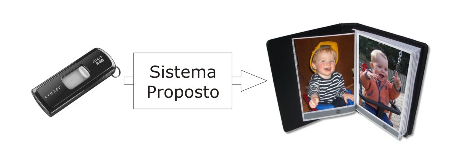
\includegraphics[scale=1]{sistemaProposto.eps}}
	\end{center}
	\caption{Sistema proposto}
	\label{fig:sistemaProposto}
\end{figure}

\begin{table}[htpb]
\begin{center}
\begin{tabular}{|c|c|c|}
\hline
coluna 1 & coluna 2 & coluna 3 \\
\hline
valor 1,1 & valor 1,2 & valor 1,3 \\
valor 2,1 & valor 2,2 & valor 2,3 \\
\hline
\end{tabular}
\end{center}
\caption{Primeira tabela.}
\label{tab:tabelaTeste}
\end{table}

\begin{equation}
E = m \times c^2
\label{eq1}
\end{equation}

\begin{lstlisting}[caption={Loop simples},label=cod1,numbers=none]
for(int x=1; x<10; x++){
  cout << x << "\n";
}
\end{lstlisting}

\section{Se\c{c}\~{a}o 2 do Capítulo 1}  
\subsection{Subseção}
\subsubsection{Subsubseção}

 
%% \input{cap2}
%!TEX root = main_mestrado.tex
\chapter{Introdução}

\begin{itemize}
	\item Comunidades de perguntas e respostas e sua importância nos dias de hoje;
	\item A importância da diversidade em uma comunidade;
	\item Desigualdade de gênero em tecnologia;
	\item Mulheres deixando o ramo antes e em maior quantidade do que homens;
	\item Razões para mulheres estarem deixando a carreira: estereótipos, unfriendlyness, falta de espaço;
	\item Consequências: mulheres não se identificam tanto, deixam de participar de comunidades de tecnologia, conteúdo enviesado;
	\item The starting motivation for this study is a preoccupation with gender diversity. More specifically, with how women participate in contributing to Social Q\&A sites. Recent results point that only a minority of contributors in StackOverflow~\cite{Vasilescu27092013}, the largest site in the StackExchange platform, are women. Moreover, recent releases of diversity information of employees in large companies like Google~\cite{google:report} and Linkedin~\cite{linkedin:report} points out that the proportion of women in tech and leadership roles are low. This result is similar to those of some online communities related to technology like FOSS communities~\cite{rustad2011suck}. Moreover, it has been reported that in StackOverflow people who question the reason for such "gender gap" may not be understood and even mistreated\footnote{http://is.gd/eAnI8R}. These facts match the common stereotyping of women in STEM related fields~\cite{spencer1999stereotype} and women's lower influence in mixed-gender groups~\cite{karpowitz2012gender}. However, if women are currently led to contribute less than men by these communities, StackExchange sites are loosing not only potential contributors, but also the chance of producing content that addresses the views of women, and ultimately of better functioning by having more mixed gender crowds~\cite{marshall1975boys}.
	\item Existem estudos de gênero em várias comunidades online, mas não nas comunidades do StackExchange como todo;
	\item Objetivo: estudar o "efeito" de identificar seu gênero em comunidades do StackExchange com relação à participação, percepção de qualidade de conteúdo, tempo de atividade no site, quantidade de contribuições ao longo do tempo e proporção de usuários ativos ao longo do tempo.
	\item Importância de estudar essas comunidades;
	\item Responder: Por que os posts das mulheres seria diferente dos feitos por homens?
	\item Mulheres tendem a se identificar menos, mas isso não é relevante, já que nós queremos ver o impacto que "ser mulher" nestas comunidades tem na participação destes usuários.
	\item Estudamos os usuários que participaram da comunidade com pelo menos uma contribuição textual (comentário, pergunta ou resposta), que possuam reputação que os permita fazer todos os tipos de contribuições textuais (50 pontos) e que tenha seu gênero facilmente identificável pelos demais usuários.
	\begin{itemize}
		\item todas as contribuições de todos os usuários que se encaixam neste padrão, desde a criação da comunidade até setembro de 2014, foram levadas em consideração para este estudo.
	\end{itemize}
	\item Esperávamos que os resultados encontrados aqui batessem com o estereótipo de que mulheres não participam de comunidades online e principalmente àquelas sobre tecnologia.
	\item Mulheres tendem a participar tanto quanto ou até mais do que homens na maioria das comunidades voltada para tecnologia. 
	\item Este resultado é importante para acabar com estereótipos e mostrar que mulheres podem e tem seu espaço garantido em comunidades online e comunidades online sobre tecnologia.
\end{itemize}

\emph{Bussiness problem}: 

\emph{Technical problem}: 

Objeto de estudo: Contribuições de um usuário durante toda a sua vida ativa nos sites de Q\&A do grupo StackExchange.

Finalidade: Definir se usuários de gêneros distintos possuem diferenças de comportamento nas comunidades estudadas.

Foco de Qualidade: (com respeito à)

Perspectiva: A perspectiva será dos próprios usuários dos sites do StackExchange. Além dos administradores, tanto da plataforma inteira, quanto de cada tema, que poderão identificar os usuários que desejam manter e incentivar na comunidade.

Contexto: Comunidades de perguntas e respostas do StackExchange criadas até Setembro de 2014.
\chapter{Revisão Bibliográfica}

\begin{itemize}
\item Male as the null gender
\end{itemize}

\begin{itemize}
	\item Mulheres são underrepresented em campos onde acredita-se que é necessário um talento inato para poder ter sucesso na área (caso de Computação e Filosofia; Neurosciência e Astronomia não)\cite{leslie2015expectations}. Já que existe o estereótipo de que mulheres não possuem tal talento\cite{tiedemann2000gender, kirkcaldy2007parental}
	\item Importante notar que não foi provado ainda que esse "talento inato" é exclusivo de homens ou mulheres.\cite{hyde2005gender}
	\item "If women internalize the stereotypes, they may also decide that these fields are not for them" \cite{wigfield2000expectancy}.
	\item 
\end{itemize}
%!TEX root = main_mestrado.tex
\chapter{Metodologia}
\label{ch:metodos}

Este capítulo detalha os dados e métodos utilizadas para medir quantidade, qualidade e frequência das contribuições dos usuários, assim como o compromisso dos usuários com a comunidade. Aqui também explicamos como identificamos os gêneros dos usuários. Todo o código utilizado neste experimento pode ser encontrado em um repositório no \emph{Github}\footnote{https://github.com/mil3na/gender-study-final}. 

\section{Dados utilizados}

Nosso estudo usa dados de todas as comunidades do \emph{StackExchange} em seu último \emph{dump} de Setembro de 2014. Contudo, para que fosse possível realizar a análise, tivemos que remover  algumas comunidades que  não possuíam atividades suficientes, por parte das mulheres, para serem analisadas. Como comunidades muito novas não apresentavam dados suficientes para serem estudados, removemos da nossa pesquisa todas as comunidades do \emph{StackExchange}, presentes no \emph{dump} de Setembro de 2014, que tenham menos de 18 meses de idade, além de comunidades que não tinham um número razoável de mulheres. A lista das 85 comunidades estudadas pode ser encontrada na Tabela~\ref{table:communities}. Mais ainda, apenas os usuários que tenham feito algum tipo de contribuição e têm, no mínimo, 50 pontos de reputação foram estudados. Esta limitação é para garantir que estudamos usuários que estiveram ativos em algum momento na comunidade estudada.

\begin{table*}[!hb]
% Tabela ficar embaixo
% \begin{tabular}{@{}ccccc@{}}
\small
\centering
\begin{tabular}{p{0.13\linewidth}p{0.16\linewidth}p{0.15\linewidth}p{0.14\linewidth}p{0.14\linewidth}p{0.10\linewidth}}
\toprule
\multicolumn{6}{c}{Comunidades Estudadas}               \\ [2pt] \midrule
academia     & cooking          & french        & magento      & productivity & spanish       \\ [2pt]
android      & crypto           & gamedev       & math         & programmers  & sqa           \\ [2pt]
anime        & cs               & gaming        & mathematica  & quant        & stackapps     \\ [2pt]
apple        & cstheory         & gardening     & mathoverflow & raspberrypi  & stackoverflow \\ [2pt]
askubuntu    & dba              & genealogy     & mechanics    & rpg          & stats         \\ [2pt]
bicycles     & diy              & german        & money        & russian      & superuser     \\ [2pt]
biology      & drupal           & gis           & movies       & salesforce   & tex           \\ [2pt]
bitcoin      & dsp              & graphicdesign & music        & scicomp      & travel        \\ [2pt]
chemistry    & electronics      & hermeneutics  & outdoors     & scifi        & unix          \\ [2pt]
chinese      & ell              & history       & parenting    & security     & ux            \\ [2pt]
christianity & english          & islam         & philosophy   & serverfault  & webapps       \\ [2pt]
codegolf     & expressionengine & japanese      & photo        & sharepoint   & webmasters    \\ [2pt]
codereview   & fitness          & judaism       & physics      & skeptics     & wordpress     \\ [2pt]
cogsci       & freelancing      & linguistics   & pm           & sound        & workplace     \\ [2pt]
\multicolumn{6}{l}{writers}       \\ [2pt]
\bottomrule
\end{tabular}
\caption[Lista de comunidades estudadas]{Lista das comunidades do \emph{StackExchange} estudadas nesta pesquisa.}~\label{table:communities}
\end{table*}

As informações utilizadas neste estudo foram obtidas no \emph{dump} trimestral\footnote{https://archive.org/details/\emph{StackExchange}} oferecido pelo \emph{StackExchange}. O grupo costuma publicar regularmente todos os dados de todos os seus sites que não contenham informações privadas do usuário (e.g. \emph{email}). Tais dados incluem perguntas, respostas e comentários postados pelos usuários, assim como os votos (positivos e negativos) recebidos por cada tipo de post. O \emph{dump} também contém a reputação de cada usuário em cada comunidade. As comunidades presentes nestes dados são classificadas pelo \emph{StackExchange} dentre estas seis categorias: \emph{Technology}, \emph{Culture/Recreation}, \emph{Life/Arts}, \emph{Science}, \emph{Business} e \emph{Professional}.

\section{Inferindo o gênero dos usuários}

Os perfis do \emph{StackExchange} não possuem explicitamente o gênero de cada usuário, já que a plataforma não exige do usuário esta informação no seu perfil. Sendo assim impossível identificar o gênero de cada usuário automaticamente, com precisão. Já que nosso objetivo neste estudo é apenas investigar o efeito de um usuário, explicitamente, manifestar seu gênero, decidimos focar apenas naqueles usuários que têm a intenção de identificar seu gênero nestas comunidades.

As comunidades do \emph{StackExchange} possuem três tipos de atividades principais: perguntar, responder e comentar. Durante a participação de um usuário nas atividades principais, só é possível identificar o gênero do seu colega por dois meios: sua foto ou nome de usuário, como pode ser visto na Figura~\ref{fig:user-reg}. Utilizamos o nome de usuário para identificar o gênero do mesmo. Sabe-se que a maioria dos usuários do \emph{StackExchange} vêm de países ocidentais, provavelmente tendo nomes típicos ocidentais~\cite{schenk2013geo}, e pesquisas anteriores mostram que, para pessoas com nomes ocidentais, inferir o gênero de uma alguém através de sue primeiro nome é um método acurado tanto para redes sociais que requerem o nome real do usuário~\cite{tang2011s}, quanto para as que não o requerem~\cite{burger2011discriminating,liu2013s}.

Nosso método de inferência de gênero é similar ao encontrado em Liu \textit{et al}.~\cite{liu2013s} e Cunha \textit{et al}.~\cite{cunha2014he}. Nós utilizamos o \emph{Global Name Data}~\cite{Hyland:2013:Online}, um banco de dados de nomes baseado em registros de nascimentos nos Estados Unidos e Reino Unido, que contém mais de 100,000 nomes únicos e a frequência com que cada nome é associado a um menino ou menina. Com este banco de dados fizemos um classificador que categoriza os usuários em três classes: Feminino, Masculino e Desconhecido, baseado na contagem de frequência probabilística de cada nome. Um usuário é classificado como Masculino se existir uma proporção significantemente maior de meninos registrados com esse nome, segundo o \emph{Global Name Data}. O gênero de um nome é considerado Desconhecido caso não haja diferença estatística entre a proporção de homens e mulheres catalogados com este nome. Nossa análise só leva em consideração aqueles usuários que possuem nomes os quais é possível inferir com confiança o gênero, de acordo com este método. Com este método, conseguimos identificar, em média, 37\% dos usuários (mínimo: 27\%, máximo: 52\%) dos usuários das comunidades estudadas. Sendo sua grande maioria homens: em média, 93\% são homens (mínimo: 74\%, máximo: 98\%). O Apêndice \ref{app:info} apresenta o sumário dos usuários identificados por gênero, em cada comunidade.

\section{Manuseio dos dados}

Os dados concedidos pelo \emph{StackExchange} são disponibilizados no formato \emph{XML}, o qual dificulta a manipulação dos mesmos. Portanto, a primeira etapa foi a inserção dos dados em um banco de dados. Como pretendíamos realizar várias associações entre as comunidades e não tínhamos um \emph{schema} fixo, optamos por um banco de dados flexível, orientado a documentos, o \emph{MongoDB}. Por praticidade, utilizamos a linguagem de programação \emph{Python} para filtrar de dentro dos arquivos \emph{XML} os dados os quais estávamos interessados, transformar no formato adequado, criar um sub banco de dados no \emph{MongoDB} para cada comunidade e inserir seus respectivos dados lá.

Próxima etapa foi filtrar os usuários que não nos interessam. Esta pesquisa foca em comportamento de usuários em um site, então os usuários que não participam da comunidade não são relevantes para o nosso estudo. Um script em \emph{Python} foi criado para remover do nosso banco de dados todos aqueles usuários que realizaram nenhuma contribuição ou que tenham uma reputação muito baixa. Consideramos uma reputação baixa aquela que não permite que um usuário possa realizar qualquer uma das principais contribuições possíveis na plataforma. Na época do estudo, o usuário precisaria de 50 pontos de reputação para poder perguntar, responder ou comentar no site.

Para cada usuário foi criada um sumário da sua participação em cada comunidade e inserido em sua entrada no banco de dados. Mais uma vez um script escrito em \emph{Python} foi utilizado para realizar esta tarefas. O sumário de cada usuário conta com o número de identificação do usuário no site, sua reputação, a data de ingresso, a média da pontuação obtida nas perguntas, respostas e comentários feitos, o número total de perguntas, respostas e comentários feitos, a taxa de aceitação e utilidade média das respostas, as datas de todas as contribuições feitas e o tipo da primeira contribuição.

\subsection{Classificando os usuários quanto ao gênero}

Para classificar os usuários quanto ao seu gênero, fizemos o \emph{download} do banco de dados oferecido pelo \emph{Global Name Data} através do site \emph{Github}\footnote{https://github.com/OpenGenderTracking/globalnamedata/tree/master/assets} e o inserimos no nosso banco de dados \emph{MongoDB}. Com um programa escrito em \emph{Python} utilizamos os dados já filtrados que se encontram em nosso banco de dados. Para cada usuário de cada site, selecionamos seu nome e verificamos se ele se encontra no banco de dados de nomes. Caso seja encontrado, inserimos a classe a qual ele pertence (Feminino, Masculino ou Desconhecido) ao seu sumário. Se não, este usuário será classificado como tendo o gênero desconhecido. Apenas os usuários que foram classificados como Feminino ou Masculino são utilizados neste estudo.

\subsection{Cálculos estatísticos}

Visto que todo a manipulação dos dados feitas até este ponto do experimento foram realizadas utilizando scripts em \emph{Python} e a não compatibilidade do banco de dados \emph{MongoDB} com a linguagem \emph{R}, na época em que o estudo foi realizado, optamos por utilizar as bibliotecas \emph{pandas}, \emph{numpy}, \emph{scipy} e \emph{statsmodels} que provêm uma funcionalidade similar a encontrada na linguagem \emph{R}. Ademais, utilizamos a ferramenta \emph{ipython notebook} que nos permite dispor código e resultados (sejam estes numéricos ou gráficos) de forma simples e clara, facilitando o entendimento e reprodução do experimento. Estes \emph{notebooks} assim como todo o código utilizado para esta pesquisa pode ser encontrado no endereço \emph{Github} citado no início deste capítulo.

\section{Medindo contribuições e engajamento}

A questão principal do nosso estudo é esclarecer o quão diferente é a participação de homens e mulheres em comunidades de perguntas e respostas, comparando àquelas relacionadas a \emph{STEM} (pertencentes às categorias \emph{Technology} e \emph{Science}) com as demais. Para responder esta questão, nós a dividimos em quatro perguntas mais específicas, que serão relatadas a seguir.

\subsection{Número de contribuições}

Nossa primeira pergunta é: \textit{O número de contribuições feitas por homens e por mulheres difere significantemente nas comunidades observadas?} Esta pergunta é relacionada aos três tipos principais de contribuição na plataforma \emph{StackExchange}: perguntas, respostas e comentários, além da soma de todas.

Como a proporção de mulheres sendo menor que a de homens na maioria dos sites das plataformas e, em alguns sites, esta proporção atingindo menos de um terço dos usuários identificados, esperávamos que isto se refletiria nas contribuições provenientes das mulheres. Em outras palavras, acreditávamos que a resposta para esta primeira pergunta seria que, independente do tipo de contribuição, mulheres contribuiriam menos do que os homens.

\subsection{Qualidade}

O controle de qualidade das perguntas e respostas na plataforma \emph{StackExchange} é feito pela própria comunidade através do sistema de votos. Usuários com uma determinada reputação podem votar "para cima" e "para baixo", caso considerem o post como uma boa ou má contribuição, respectivamente. Esses votos geram pontos, positivos ou negativos, que, dentre outros fatores, formam a reputação de um usuário. 

Tendo em vista o processo de avaliação de qualidade descrito acima, a nossa segunda pergunta é: \textit{As contribuições feitas por diferentes gêneros são vistas, pela comunidade, com níveis de qualidade diferentes?} Caso exista uma avaliação negativa indiscriminada das contribuições provenientes de mulheres, elas podem estar contribuindo menos porque suas contribuições não são bem provenientes, fazendo com que elas sintam que falharam e as desencorajando de continuar participando. 

Utilizamos a pontuação criada pelo sistema de votos para medir a qualidade das perguntas e respostas de cada usuário. A qualidade das perguntas de um usuário é definida como a média da pontuação de todas as perguntas feitas pelo usuário, ou zero, caso o usuário tenha contribuído com nenhuma pergunta. Para respostas, utilizamos duas métricas: a primeira é a taxa de aceitação que mede a proporção de respostas do usuário que foram aceitas como melhor resposta pelo interrogador. A segunda é a utilidade média das respostas, proposta por Furtado \textit{et al}.~\cite{furtado2013contributor}. Esta métrica é a média da normalização do saldo de votos das respostas de um usuário comparado com outras respostas à mesma pergunta. Para ambas as métricas para respostas, apenas usuários com pelo menos uma resposta são levados em consideração.

\subsection{Engajamento}

Neste estudo, usamos a definição de engajamento a qual o descreve como o esforço de um usuário ao longo do tempo. Nós medimos engajamento tanto em relação ao tempo total que o usuário permanece na comunidade (seu tempo de vida) quanto sua frequência de contribuição durante seu tempo de atividade.

Levando em consideração estas definições, nossa terceira pergunta é: \textit{O engajamento de homens e mulheres difere nas comunidades estudadas?} É importante notar que, caso haja diferença no hábito de contribuição entre homens e mulheres, podemos verificar se usuários de algum dos gêneros deixam a comunidade mais cedo ou têm uma taxa de contribuição menor, nos ajudando a entender melhor as diferenças (ou similaridades) entre homens e mulheres com relação ao seus hábitos de contribuição.

O tempo de vida de um usuário em uma comunidade do \emph{StackExchange} não pode ser considerado apenas como a diferença entre a data de sua primeira contribuição e a última. Já que uma pergunta (e suas respectivas respostas) podem ser transferidas entre comunidades\footnote{http://meta.stackExchange.com/questions/2683/move-questions-between-stack-exchange-sites}. Desse modo, definimos a seguir o tempo de vida de um usuário em uma determinada comunidade. 

Antes de tudo, definimos o primeiro dia de atividade do usuário como a data mais recente entre o dia de cadastro do usuário e a data da sua primeira contribuição na comunidade. Esta medida evita que levemos em consideração um período que o usuário não esteve ativo na comunidade em questão, mas esteve em outra comunidade e sua pergunta foi transferida. Mais ainda, definimos que um usuário está inativo quando ele não produz nenhuma contribuição por um período de tempo maior que o intervalo de morte da comunidade. Este intervalo, medido em dias, é calculado da seguinte maneira: para cada usuário obtemos o maior intervalo entre duas de suas contribuições consecutivas. O intervalo de morte é a média dos maiores intervalos de todos os usuários. Por fim, o tempo de vida de um usuário é a diferença entre a data da sua última contribuição e a data da sua primeira atividade(ou cadastro), medida em dias.

A frequência de participação, segunda métrica usada nesta pergunta, é definida como o total de contribuições feita por um usuário (perguntas, respostas ou comentários) dividido pelo número de dias nos quais o usuário estava ativo. Ao contrário do tempo de vida, aqui nós consideramos apenas os dias em que o usuário contribuiu para a comunidade.

A nossa expectativa para a resposta desta pergunta era que mulheres se engajam menos, principalmente às comunidades que abordam assuntos relacionados a \emph{STEM}. Existe um estigma de que estas comunidades não são atrativas às mulheres e que também são excludentes, fazendo com que mulheres não sejam bem-vindas. Por esses motivos, as poucas mulheres que se cadastrasse em qualquer site o deixaria em pouco tempo.

\subsection{Contribuições e registros ao longo do tempo}

Para esta pergunta, verificamos se a falta de contribuição por parte das mulheres é algo novo nestas comunidades, ou ainda se existem padrões de contribuição ao longo do tempo, seja de aumento ou redução. Investigamos também se existe alguma tendência no número de registros feito por cada gênero. Em outras palavras, buscamos responder à seguinte pergunta: \textit{A proporção de contribuições e registros feitos por usuários de cada gênero tem aumentado ou reduzido ao longo do tempo?}. 

Se mulheres contribuem pouco e por pouco tempo é lógico esperar que a proporção de contribuições por parte das mulheres tenha aumentado por um tempo, mas estagnado depois e, provavelmente até diminuído nos últimos meses. O mesmo é o que esperamos para a proporção de registros, até porque estas comunidades são conhecidas por não serem \emph{female-friendly}.

\section{Distribuições e testes}

A maioria das variáveis possuem uma distribuição bastante enviesada e com certeza não normal, como pode ser visto no Apêndice~\ref{app:distrib}. Portanto, utilizamos testes não paramétricos. Para comparar o número de contribuições (e de cada tipo de contribuição), a qualidade das contribuições e a frequência de contribuição de cada gênero utilizamos o teste um teste de dominância estocástica, o \emph{Mann-Whitney-U} não pareado. Primeiramente a versão bilateral do teste para verificar se há diferença estatística e, em seguida, o mesmo teste é aplicado aos grupos que apresentaram diferença estatística mas, desta vez, utilizando sua versão unilateral para verificar se o grupo de mulheres era o que apresentava dominância estocástica.

Para testar se homens e mulheres possuem um tempo de vida divergente na comunidade utilizamos a \textit{Survival Analysis} junto com um teste \emph{LogRank}. Já para a quarta pergunta tomamos a proporção de contribuição e registros feitos por cada grupo de gênero, a cada seis meses, e verificamos se esta proporção aumenta ou não, com a ajuda de uma regressão utilizando o método dos mínimos quadrados.

Sumário das variáveis estudadas, para cada pergunta de pesquisa, podem ser encontrados nos Apêndices~\ref{app:q1},~\ref{app:q2},~\ref{app:q3} e ~\ref{app:q4}.

% section methods (end)


%!TEX root = main_mestrado.tex
\chapter{Resultados}

%!TEX root = proceedings.tex
\section{Results} % (fold)
\label{sec:results}

\begin{figure}
  \raggedleft
  \includegraphics[width=1\columnwidth]{figures/questions_women.pdf}
  \caption{Comparison of the number of questions posted by contributors of different gender in sites where a significant difference was identified and women contribute with more questions. The box represents the quartiles of the distributions, while the whiskers show the 1st and 99th percentile values. Recall that a MMW test may find significant difference in rank sum even if some of the quartiles are similar for the two samples. For visualizing the distributions on a log scale, the value we display is the number of contributions of each user plus one. }~\label{figure:questions}
\end{figure}

This section presents the results for each of the four questions we address. When describing the differences in a variable for a set of sites, we use the notation $W/S/M$, with $W$ being the number of sites in which women had significantly higher values for that variable, $S$ the number of sites with no significant difference, and $M$ the number of sites in which men had significantly higher values.  

\subsection{Number of contributions}
For all four types of contribution considered, a common pattern emerges in our results: the amount of contributions from men and women is not significantly different in the majority of sites (Mann-Whitney-Wilcoxon U significance tests, $\alpha = 0.05$). % [n] Show this result. TODO

For all types of contribution, when there are differences in contribution levels, there is larger number of sites in which a typical women contributor is more active than sites in which men tend to contribute more. The difference in this number is the highest for questions ($21/62/2$), followed by answers ($18/56/11$) and all contributions combined ($10/73/2$). 

\begin{figure}
  % \centering
  \raggedleft
  \includegraphics[width=1\columnwidth]{figures/answers_women.pdf}
  \caption{Comparison of the number of answers posted by contributors of different gender in sites where a significant difference was identified and women contribute with more answers. The box represents the quartiles of the distributions, while the whiskers show the 1st and 99th percentile values. For visualizing the distributions on a log scale, the value we display is the number of contributions of each user plus one. }~\label{figure:answers}
\end{figure}

Interestingly, the categories in which these differences happen differ for answers in contrast with the other types of contribution. For questions, comments, and all contributions combined, the communities where women are usually more active are related to STEM categories. For questions, this distribution is $16/28/0$ for the STEM sites, as seen in Figure~\ref{figure:questions}. In contrast, when considering answers, only three of the 18 sites in which women tend to answer more are STEM sites (see Figure ~\ref{figure:answers}). Most often, sites in which women answer significantly more than men happen in the life-arts or professional categories. Also, two of the three STEM sites in which women answer more are stereotypically associated with women: UX and Software Quality Assurance. The other way around, communities which men answer more than women can be seen on Figure~\ref{figure:answers-men}.

\begin{figure}
  % \centering
  \raggedleft
  \includegraphics[width=1\columnwidth]{figures/answers_men.pdf}
  \caption{Comparison of the number of answers posted by contributors of different gender in sites where a significant difference was identified and men contribute with more questions. The box represents the quartiles of the distributions, while the whiskers show the 1st and 99th percentile values. For visualizing the distributions on a log scale, the value we display is the number of contributions of each user plus one. }~\label{figure:answers-men}
\end{figure}

These results point that women who engage with most sites we study and display their gender usually do not contribute significantly less than men. In fact, when there are differences, they are most often on the opposite direction. 
%The communities in which difference happen, however, 

\subsection{Quality evaluation} % (fold)
\label{subsec:qualidade}
Few sites display a significant difference in how they evaluate the quality of contributions made by men and women. This difference happens less often than a difference in number of contributions. For the acceptance ratio ($7/76/2$) and mean utility of answers ($9/74/2$) from users, slightly more communities tend to attribute higher quality of the answers from women. For the average voting balance of questions posted, there is an equilibrium in the sites we study ($8/67/10$). Moreover, there seems to be no clear trend in the sites regarding the categories in which significant differences in quality evaluation happen. 

% section qualidade (end)



\subsection{Engagement}% (fold)
For the metrics that consider time, the differences that we observe have a clear trend. First, for most sites, there is no significant difference in the lifetime of activity frequency of men and women. However, when differences in lifetime occur, they happen more often because men stay for longer in a community than the opposite ($1/70/14$). Conversely, the frequency of contributions in active days happens more often because women are more active than the other way around ($10/74/1$). 

We also observe that the largest difference in lifetime occurs in StackOverflow, the the most popular and oldest site in StackExchange. Moreover, the following three sites with largest differences in lifetime are also old and STEM-related: MathOverflow, SuperUser and ServerFault, See Table~\ref{table:lifetime}. 

\begin{table}[h]
\centering
\begin{tabular}{@{}rllr@{}}
\toprule
{\small\textit{Median Diff.}} & {\small \textit{Category}} & {\small \textit{Community}} & {\small \textit{Age (mon) }} \\ \midrule
-346.87                            & technology         & stackoverflow      & 76                 \\ \midrule
-327.76                           & science            & mathoverflow       & 62                 \\ \midrule
-70.93                            & technology         & superuser          & 64                 \\ \midrule
-35.29                            & technology         & serverfault        & 67                 \\ \midrule
-17.15                            & technology         & dsp                & 39                 \\ \midrule
-14.50                            & technology         & apple              & 51                 \\ \midrule
-12.62                            & life-arts          & diy                & 52                 \\ \midrule
-9.05                             & culture-recr. & english            & 51                 \\ \midrule
-8.80                             & life-arts          & scifi              & 46                 \\ \midrule
-7.26                             & technology         & networkengineering & 18                 \\ \midrule
-6.42                             & culture-recre. & mechanics          & 44                 \\ \midrule
-4.98                             & life-arts          & photo              & 52                 \\ \midrule
-1.92                             & culture-recre. & travel             & 41                 \\ \midrule
-1.66                             & science            & philosophy         & 41                 \\ \midrule
\textbf{74.72}                             & technology         & wordpress          & 51                 \\ \bottomrule
\end{tabular}
\caption{Sites where we can see a significant difference, the median difference in days and it's age, in months}~\label{table:lifetime}
\end{table}

For frequency, a different pattern happens. In all seven STEM sites for which there is a difference in the frequency of activity, women have a higher frequency than men. Together with the lifetime results, this suggests that although women leave the community sooner than men, they act more while they are still engaged with the community.


\subsection{Contributions and registrations over time}
For the dynamics of contributions coming from men and women, we see that in roughly a quarter of the sites, the fraction of contributions coming from women is increasing ($20/60/5$). Albeit less pronounced, for the communities where proportion of registrations from different genders have a significant trend over time, it happens more often that the number of registrations coming from women is increasing: $8/76/1$. Both of these trends are also stronger considering only STEM sites: $16/25/3$ for contributions over time, and $6/38/0$ for proportion of new registrations.



\subsection{A zoom in the largest sites} %  DEixamos essa seção? Retirada.
The two largest sites of StackExchange -- StackOverflow and SuperUser -- are much larger and older than the remainder sites in our data. Because they thus own a significant proportion of all StackExchange users, we highlight their behavior. In both sites, there men have significantly longer lifetimes, and answers more questions. On the other hand, the proportion of new registrations coming from women has increased over time. 

A comparison of  the number of contributions on the top five bigger StackExchange communities related to STEM can be seen on Figure~\ref{figure:top-five}.



\begin{figure}
  % \centering
  % \raggedleft
  \includegraphics[width=1\columnwidth]{figures/five-largest_quantity.pdf}
  \caption{Comparison of the number of contributions posted by users of different gender in the five biggest (in user count, ordered from the most populous to the least) related to STEM on StackExchange. The box represents the quartiles of the distributions, while the whiskers show the 1st and 99th percentile values. }~\label{figure:top-five}
\end{figure}
% section conclusions (end)

% section tempo (end)


% section results (end)


%!TEX root = main_mestrado.tex
\chapter{Discussão}
\label{ch:discussao}

Neste capítulo iremos comentar os resultados obtidos no nosso experimento e associá-los à literatura relacionada ao estudo aqui descrito. Dividimos nossos resultados entre as semelhanças e diferenças encontradas e, apesar da importância do primeiro tópico, focamos nas diferenças por estas serem mais controversas.

\section{As semelhanças}

Nossa expectativa ao observar contribuições individuais de usuários de diferentes gêneros era que mulheres, por serem uma minoria, iriam participar menos destes sites, assim como na \emph{Wikipedia}~\cite{antin2011gender} e comunidades \emph{FOSS}~\cite{rustad2011suck}. Contudo, o que encontramos não foram diferenças, mas uma grande equivalência entre o comportamento de homens e mulheres nos sites estudados. 

No geral, saber que mulheres contribuem de maneira similar aos homens na maioria dos sites aponta que uma mulher que se cadastrar em um site aleatório do \emph{StackExchange} provavelmente irá encontrar um ambiente que não a estimule a contribuir menos ou menos frequentemente que os homens. Tal resultado é animador visto que, apesar da pequena proporção de mulheres nestas comunidades, o comportamento das mesmas não segue a linha das pesquisas anteriores onde mulheres contribuem menos que homens quando estão em minoria.

\section{As diferenças}

Tendo em mente todo o estereótipo em \emph{STEM} que mulheres são enquadradas, esperávamos que sua baixa representatividade também representaria baixa contribuição. Ademais, esperávamos que o estereótipo de mulheres em tecnologia~\cite{hyde1990gender} e aquele em que mulheres não possuem um taleto inato para ciência~\cite{leslie2015expectations} fosse influenciar na opinião que os outros usuários teriam das suas colegas, fazendo com que mulheres recebessem \emph{feedback} negativo nas suas contribuições, indiscriminadamente, levando o conteúdo das mulheres a serem classificados com menor qualidade pela comunidade. Sem esquecer que outros estudos já tinham identificado o conteúdo vindo de mulheres como de qualidade inferior comparado ao de homens, tanto em tarefas de matemática~\cite{campbell1986effects} quanto em comunidades online~\cite{collier2012conflict}.

Contudo, não é isso que acontece. Na maioria dos sites, mulheres produzem conteúdo de tão boa qualidade quanto homens, segundo a visão da comunidade. Vemos que estas mulheres contribuem bastante com perguntas e comentários, tendo uma frequência de contribuições muitas vezes maior que a de homens. 

% Por outro lado, apesar de mulheres respondem mais do que homens em várias comunidades, quando observamos apenas comunidades relacionadas a \emph{STEM} esta proporção é invertida. Inclusive, mulheres respondem menos nos quatro maiores e mais antigos sites da plataforma: StackOverflow, SuperUser, SeverFault e Mathematics. Mais ainda, em praticamente todas as comunidades que observamos diferença estatística quanto ao tempo de vida, homens passavam mais tempo na comunidade.

% Quanto ao tempo de vida de mulheres nestas comunidades, nota-se que a diferença de tempo é maior em comunidades mais antigas, vide tabela \ref{table:lifetime}. Isso pode se dar por que tais comunidades, a exemplo do StackOverflow, foram criadas por um grupo de homens e se mantiveram assim por bastante tempo, até se tornarem popular. Este grupo de usuários provavelmente tem um tempo de vida bem maior do que as mulheres que eventualmente ingressaram na comunidade. 

Por outro lado, apesar de mulheres responderem mais do que homens em várias comunidades, quando observamos apenas comunidades relacionadas à \emph{STEM} isto não acontece. Mulheres contribuem com menos respostas do que homens em todos os quatro maiores e mais antigos sites da plataforma: \emph{StackOverflow}, \emph{SuperUser}, \emph{SeverFault} e \emph{Mathematics}. Se estes sites influenciam mulheres a participar menos no processo de resposta, a grandeza deles pode implicar que um grande número de mulheres está contribuindo com menos respostas do que poderia estar. Sabendo que existem sites em outras categorias nas quais mulheres comuns respondem mais do que homens, nossos resultados sugerem que há um fator característico em alguns sites -- e provavelmente à comunidade -- atuando no comportamento das mulheres quanto às suas contribuições. A ampla diferença no tempo de vida entre homens e mulheres nestas comunidades complementa este pensamento (ver Tabela~\ref{table:lifetime}).

Uma característica comum a algumas comunidades relacionadas à \emph{STEM} do \emph{StackExchange} é que elas são ramos do \emph{StackOverflow} que foi criada por um grupo de homens e se manteve assim por bastante tempo, até se tornar popular. É provável que este grupo de homens tenha sua própria cultura dentro do \emph{StackOverflow}, com seus valores e práticas que não sejam amigáveis às mulheres, e esta cultura tenha passado para os demais sites, fazendo com que estes sejam sites com características sociais que não atraiam as mulheres.

Nosso resultado se alinha com o de Yang \textit{et al}.~\cite{yang2010activity}, que apesar de não estudar a mesma comunidade de perguntas e respostas, defendeu que usuários que têm o tempo de vida maior na comunidade preferem responder à perguntar. No nosso estudo, verificamos que estes usuários são geralmente homens, assim como entenderam Vasilescu \textit{et al}.~\cite{Vasilescu27092013}. Vasilescu \textit{et al} consideram este resultado insalubre para a comunidade, visto que bons contribuidores estão deixando a comunidade. Nós acreditamos que exista uma barreira para que mulheres continuem contribuindo, podendo ser desde a aquisição, por parte delas, do pensamento de que não são capazes de contribuir, até por perseguições/assédios dentro da própria comunidade por parte dos outros usuários. Estas hipóteses, contudo, pedem uma investigação mais detalhada, fora do escopo desta pesquisa.

Apesar de não ser relacionada com sua real performance, a percepção que uma pessoa tem de sua capacidade cognitiva em um campo influencia como esta pessoa acha que se sairá em uma determinada tarefa. No mais, achar que não vai se dar bem em uma tarefa pode fazer com que, caso seja dada a opção, a pessoa não chegue a tentar realizar tal atividade. Mulheres acham que não são boas em tarefas sobre ciência e isso as influencia a não participar do campo~\cite{ehrlinger2003chronic}. Isso pode explicar porque a proporção de mulheres é tão baixa nas comunidades sobre \emph{STEM}, mas elas se dão tão bem quanto homens na maioria delas.

% Uma justificativa para mulheres responderem menos em comunidades de \emph{STEM} pode ser a de que respostas podem ser consideradas mais competitivas do que perguntas. Afinal, todas as respostas passam por um "processo seletivo" para ser a melhor resposta de uma determinada pergunta, o que não acontece com perguntas nem comentários. Já se sabe que mulheres não se dão bem em ambientes competitivos, principalmente quando precisam competir com homens~\cite{gneezy2003performance}, e tendem a evitá-los~\cite{niederle2005women,croson2009gender}. Além de que, demonstrar conhecimento em um assunto desta área pode exigir uma auto-confiança no campo que mulheres não têm.

Se olharmos para comunidades de áreas de \emph{STEM} que são conhecidas por terem mais mulheres, observamos que o resultado é similar aos de comunidades não relacionadas à \emph{STEM}. Tomando como exemplo a comunidade \emph{UX} (\textit{user experience}), cujas variáveis podem ser observadas na Figura~\ref{fig:ux}, mulheres respondem mais nesta comunidade, o que pode ser uma demonstração de auto confiança no seu conhecimento no assunto. Mais ainda, \emph{UX} não é considerada uma disciplina que necessita de um conhecimento inato para ter sucesso na área, sendo este mais um motivo para mulheres não se inibirem em participar desta comunidade de todas as formas possíveis. 

\begin{figure}
  \centering
  \includegraphics[height=0.65\paperheight]{figures/ux.pdf}
  \caption[Distribuição das variáveis para o site \emph{User Experience}]{Distribuição das variáveis para o site \emph{User Experience}. Mostramos um histograma do log do valor da variável mais um para as variáveis discretas e a gráfico da função de densidade, para as variáveis contínuas.}~\label{fig:ux}
\end{figure}

Ver que mulheres têm aumentado sua proporção de contribuições ao longo do tempo, principalmente em comunidades sobre assuntos relacionados à \emph{STEM}, nos dá uma esperança de que a barreira que existe para que mulheres entrem e contribuam para estas comunidades esteja diminuindo. Já que outras comunidades, como as comunidades \emph{FOSS}~\cite{powell2010gender}, mulheres que já estão envolvidas tendem a continuar fazendo parte dela. Uma maneira de aumentar a autoconfiança destas mulheres quanto ao seu conhecimento também é essencial para aumentar estas proporções, já que elas mesmas consideram ter autoconfiança algo essencial para se manter em comunidades nas quais elas são maioria~\cite{powell2010gender}.

No geral, nossos resultados mostram que a maioria dos sites do \emph{StackExchange} possui comunidades com poucas diferenças de comportamento relacionadas ao gênero. Porém, conseguimos enxergar claramente duas barreiras para a participação de mulheres nestes sites: uma na entrada, considerando a baixa proporção de contribuidoras e outra relacionada à partida antecipada de mulheres engajadas. Ambas as barreiras são mais expressivas nas maiores comunidades relacionadas à \emph{STEM}, sugerindo que nestas comunidades, mulheres sentem ainda mais dificuldade em participar. Todos esses pensamentos, juntamente com o fato de que mulheres tendem a contribuir com mais perguntas do que homens nestas comunidades, requerem uma investigação qualitativa aprofundada de modo a entender por que este padrão existe.


% Esse parágrafo é interessante, mas não acho que cabe aqui.
% However, in Wikipedia, it has been found that women are more likely to be involved in social- and community-oriented areas of the site~\cite{lam2011wp}. This is in line with women being more likely to comment in the communities we study, where comments are the primarily means of socialization. Nevertheless, the higher likelihood of women to produce questions in three of the communities remains an open question for future work. A possible explanation to be considered is that self-selection leads more men contribute as answering-only users in these communities.

% \subsection{Discussão do design}

% O que nosso estudo deixa bem claro é que as comunidades do \emph{StackExchange} possuem duas barreiras para a contribuição por parte das mulheres: um para que elas entrem e comecem a participar da comunidade e outra para que elas permaneçam tanto tempo quanto seus colegas do sexo masculino. As comunidades do \emph{StackExchange} pode estar perdendo muito, em termos de conteúdo, com essa postura por parte das mulheres em seu sites.

% É provável que exista preconceito e perseguição dentro destas comunidades sim, assim como boa parte das comunidades onlines. Identificar e eliminar usuários que não têm um comportamento de acordo com os termos da comunidade é uma boa prática. Contudo, é necessário mostrar para as mulheres que isto está sendo feito, para que elas possam se sentir seguras neste ambiente. 

% Mais ainda, uma campanha feminista (lembrando que o feminismo promove a igualdade entre os sexos e não a dominação do sexo feminino) para promover o site pode ser um bom primeiro contato com a comunidade feminina e procurar saber diretamente delas como melhorar.

% subsection sugestoes (end)


% Note to self: estou começando a achar que existe prejudice e harassment sim, mas as mulheres que conseguem se engajar com estas comunidades de tecnologia conseguem ignorar essas negatividades. Newcomers podem ver isto como barreira e nem se quer entrar na comunidade.

% "StackOverflow was founded by men, and this community may continued as a group of men until reach a certain popularity, number of users and before the birth of \emph{StackExchange} along with other communities, as most of them come from branches of StackOverflow. "

% "This pattern of data suggests, by extension, that women might disproportionately avoid scientific pursuits because their self-views lead them to mischaracterize how well they are objectively doing on any given scientific task. Because they think they are doing more poorly than do men, they are more likely than men to avoid science when given an option." Texto de ehrlinger2003chronic
%!TEX root = main_mestrado.tex
\chapter{Conclusões}

\begin{itemize}
	\item Parágrafo resumindo o que foi feito e um pouco dos resultados;
	\item Parágrafo sobre confidence e como isso pode ter influenciado na participação de mulheres e nos resultados que encontramos;
	\item Parágrafo comparando o resultado que achamos com o resultado em outras comunidades;
	\item Parágrafo falando como este estudo pode ajudar no gender gap problem;
	\item Como este trabalho pode ajudar a melhorar as comunidades?
	\item Falar sobre trabalhos futuros;
	\item Já se sabe que pessoas podem ser influenciadas quanto à maneira que elas acham que vão se sair em uma certa task e que isto pode influenciar na sua vontade de participar de algo \cite{ehrlinger2003chronic}. É possível que estes resultados mudem a percepção de mulheres sobre sua participação no site e as faça participar mais.
\end{itemize}
% \chapter{Introdu\c{c}\~{a}o}

\section{Se\c{c}\~{a}o 1 do Capítulo 1}
\subsection{Subseção}
\subsubsection{Subsubseção}

% A Figura \ref{fig:sistemaProposto}. A Tabela \ref{tab:tabelaTeste}. A Equação (\ref{eq1}). O trabalho de fulano~\cite{ref1}. O Código Fonte \ref{cod1}.

\begin{figure}[htbp]	
\begin{center}
		\fbox{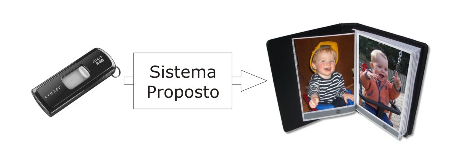
\includegraphics[scale=1]{sistemaProposto.eps}}
	\end{center}
	\caption{Sistema proposto}
	\label{fig:sistemaProposto}
\end{figure}

\begin{table}[htpb]
\begin{center}
\begin{tabular}{|c|c|c|}
\hline
coluna 1 & coluna 2 & coluna 3 \\
\hline
valor 1,1 & valor 1,2 & valor 1,3 \\
valor 2,1 & valor 2,2 & valor 2,3 \\
\hline
\end{tabular}
\end{center}
\caption{Primeira tabela.}
\label{tab:tabelaTeste}
\end{table}

\begin{equation}
E = m \times c^2
\label{eq1}
\end{equation}

\begin{lstlisting}[caption={Loop simples},label=cod1,numbers=none]
for(int x=1; x<10; x++){
  cout << x << "\n";
}
\end{lstlisting}

\section{Se\c{c}\~{a}o 2 do Capítulo 1}  
\subsection{Subseção}
\subsubsection{Subsubseção}




%%%%%%%%%%%%%%%%%%%%%%%%%%%%%%%%%%%%%%%%%%%%%%%%%%%%%%%%%%%%%%%%%%%%%%%%%%%%%%%%
%% Bibliografia
%% Coloque suas referencias no arquivo ref.bib e descomente as proximas duas linhas

\bibliographystyle{plain} % estilo de bibliografia   plain,unsrt,alpha,abbrv.
\bibliography{ref} % arquivos com as entradas bib.

%%%%%%%%%%%%%%%%%%%%%%%%%%%%%%%%%%%%%%%%%%%%%%%%%%%%%%%%%%%%%%%%%%%%%%%%%%%%%%%%
%% Apendice
% Caso seja necessario algum apendice, descomente a proxima linha.

\appendix
%!TEX root = ../main_mestrado.tex

\chapter{Sumário dos usuários identificados}
\label{app:info}
\small
\begin{longtabu}{@{}
	p{0.17\linewidth}
	p{0.2\linewidth}
	P{0.1\linewidth}
	P{0.1\linewidth}
	P{0.1\linewidth}
	P{0.1\linewidth}
	p{0.15\linewidth}@{}}
\toprule
\textit{Comunidade}  & \textit{Categoria}    & \textit{Idade (meses)} & \textit{Número Homens} & \textit{Número Mulheres} & \textit{Proporção Identif.} \\ \midrule
\endhead

\\ \hline
\endfoot

\\
\endlastfoot

academia         & life-arts          & 33    & 1124             & 99      & 34.41\%     \\
android          & technology         & 50    & 2828             & 166     & 35.05\%     \\
anime            & culture-recreation & 23    & 193              & 28      & 27.80\%     \\
apple            & technology         & 51    & 5321             & 210     & 38.20\%     \\
askubuntu        & technology         & 52    & 9502             & 430     & 33.75\%     \\
bicycles         & culture-recreation & 51    & 907              & 38      & 40.18\%     \\
biology          & science            & 35    & 617              & 70      & 36.50\%     \\
bitcoin          & business           & 39    & 815              & 29      & 35.63\%     \\
chemistry        & science            & 31    & 400              & 36      & 33.72\%     \\
chinese          & culture-recreation & 35    & 245              & 22      & 29.70\%     \\
christianity     & culture-recreation & 39    & 632              & 41      & 40.49\%     \\
codegolf         & technology         & 46    & 1637             & 63      & 34.16\%     \\
codereview       & technology         & 46    & 4046             & 155     & 35.96\%     \\
cogsci           & science            & 34    & 312              & 32      & 38.10\%     \\
cooking          & life-arts          & 52    & 1602             & 202     & 39.05\%     \\
crypto           & technology         & 40    & 653              & 29      & 35.65\%     \\
cs               & science            & 32    & 969              & 53      & 35.96\%     \\
cstheory         & science            & 51    & 1107             & 51      & 44.11\%     \\
dba              & technology         & 46    & 3268             & 127     & 38.32\%     \\
diy              & life-arts          & 52    & 1613             & 70      & 41.31\%     \\
drupal           & technology         & 44    & 1372             & 108     & 33.19\%     \\
dsp              & technology         & 39    & 460              & 32      & 32.50\%     \\
electronics      & technology         & 50    & 2505             & 92      & 34.65\%     \\
ell              & culture-recreation & 22    & 704              & 67      & 34.04\%     \\
english          & culture-recreation & 51    & 5348             & 441     & 37.66\%     \\
expressionengine & technology         & 24    & 358              & 27      & 51.96\%     \\
fitness          & life-arts          & 44    & 734              & 63      & 37.23\%     \\
freelancing      & professional       & 18    & 159              & 21      & 39.22\%     \\
french           & culture-recreation & 39    & 321              & 33      & 34.10\%     \\
gamedev          & technology         & 52    & 2803             & 128     & 34.43\%     \\
gaming           & culture-recreation & 52    & 3671             & 201     & 32.28\%     \\
gardening        & life-arts          & 41    & 433              & 61      & 40.86\%     \\
genealogy        & life-arts          & 25    & 108              & 39      & 52.50\%     \\
german           & culture-recreation & 42    & 499              & 44      & 34.13\%     \\
gis              & technology         & 52    & 1757             & 159     & 36.33\%     \\
graphicdesign    & life-arts          & 46    & 1497             & 110     & 36.37\%     \\
hermeneutics     & culture-recreation & 37    & 211              & 20      & 43.02\%     \\
history          & culture-recreation & 37    & 495              & 41      & 38.31\%     \\
islam            & culture-recreation & 29    & 231              & 21      & 35.80\%     \\
japanese         & culture-recreation & 42    & 271              & 32      & 30.27\%     \\
judaism          & culture-recreation & 42    & 374              & 38      & 36.69\%     \\
linguistics      & science            & 38    & 327              & 25      & 37.13\%     \\
magento          & technology         & 22    & 488              & 37      & 39.89\%     \\
math             & science            & 52    & 9568             & 808     & 34.57\%     \\
mathematica      & technology         & 34    & 857              & 63      & 36.05\%     \\
mathoverflow     & science            & 62    & 3965             & 283     & 52.69\%     \\
mechanics        & culture-recreation & 44    & 575              & 25      & 37.90\%     \\
money            & life-arts          & 51    & 1356             & 81      & 38.79\%     \\
movies           & life-arts          & 36    & 712              & 52      & 34.82\%     \\
music            & life-arts          & 43    & 788              & 52      & 36.05\%     \\
outdoors         & culture-recreation & 34    & 269              & 24      & 37.76\%     \\
parenting        & life-arts          & 44    & 702              & 114     & 41.30\%     \\
philosophy       & science            & 41    & 623              & 32      & 37.88\%     \\
photo            & life-arts          & 52    & 1729             & 99      & 39.64\%     \\
physics          & science            & 48    & 2992             & 165     & 35.79\%     \\
pm               & business           & 45    & 609              & 40      & 41.93\%     \\
productivity     & life-arts          & 41    & 619              & 58      & 35.90\%     \\
programmers      & technology         & 50    & 9812             & 415     & 39.20\%     \\
quant            & business           & 46    & 402              & 24      & 35.32\%     \\
raspberrypi      & technology         & 29    & 858              & 28      & 35.44\%     \\
rpg              & culture-recreation & 51    & 889              & 67      & 32.92\%     \\
russian          & culture-recreation & 29    & 168              & 20      & 34.75\%     \\
salesforce       & technology         & 28    & 574              & 41      & 41.41\%     \\
scicomp          & science            & 36    & 453              & 23      & 38.76\%     \\
scifi            & life-arts          & 46    & 2058             & 216     & 37.03\%     \\
security         & technology         & 48    & 3065             & 127     & 36.14\%     \\
serverfault      & technology         & 67    & 16627            & 571     & 37.64\%     \\
sharepoint       & technology         & 43    & 1448             & 92      & 42.44\%     \\
skeptics         & culture-recreation & 45    & 1238             & 80      & 38.41\%     \\
sound            & technology         & 48    & 381              & 21      & 43.55\%     \\
spanish          & culture-recreation & 36    & 267              & 22      & 37.39\%     \\
sqa              & technology         & 42    & 423              & 35      & 44.81\%     \\
stackapps        & technology         & 56    & 509              & 24      & 40.63\%     \\
stackoverflow    & technology         & 76    & 149340           & 9806    & 35.50\%     \\
stats            & science            & 52    & 2512             & 200     & 36.01\%     \\
superuser        & technology         & 64    & 21331            & 931     & 36.21\%     \\
tex              & technology         & 52    & 4321             & 340     & 36.94\%     \\
travel           & culture-recreation & 41    & 1240             & 114     & 37.64\%     \\
unix             & technology         & 51    & 5086             & 218     & 33.42\%     \\
ux               & technology         & 51    & 3324             & 242     & 40.09\%     \\
webapps          & technology         & 53    & 2990             & 170     & 37.72\%     \\
webmasters       & technology         & 52    & 3042             & 175     & 38.88\%     \\
wordpress        & technology         & 51    & 2700             & 184     & 38.39\%     \\
workplace        & professional       & 31    & 1441             & 140     & 36.72\%     \\
writers          & life-arts          & 48    & 620              & 70      & 40.66\%  \\ \bottomrule

\caption[Sumário dos usuários identificados]{Sumário mostrando, para cada comunidade, sua categoria, sua idade, em meses, o número total de homens e mulheres identificados e a proporção de usuários que conseguimos identificar.}
\end{longtabu}
%!TEX root = ../main_mestrado.tex
\chapter{Distribuição das variáveis das cinco maiores comunidades}
\label{app:distrib}

\begin{figure}
  \centering
  \includegraphics[height=0.65\paperheight]{figures/stackoverflow.pdf}
  \caption[Distribuição das variáveis para o site \emph{StackOverflow}]{Distribuição das variáveis onde foi aplicado o teste \emph{Mann-Whitney-U} para o site \emph{StackOverflow}. Mostramos um histograma do log do valor da variável mais um para as variáveis discretas e a gráfico da função de densidade, para as variáveis contínuas. }
\end{figure}

\begin{figure}
	\centering
  \includegraphics[height=0.65\paperheight]{figures/superuser.pdf}
 \caption[Distribuição das variáveis para o site \emph{SuperUser}]{Distribuição das variáveis onde foi aplicado o teste \emph{Mann-Whitney-U} para o site \emph{SuperUser}. Mostramos um histograma do log do valor da variável mais um para as variáveis discretas e a gráfico da função de densidade, para as variáveis contínuas. }
\end{figure}

\begin{figure}
	\centering
  \includegraphics[height=0.65\paperheight]{figures/serverfault.pdf}
  \caption[Distribuição das variáveis para o site \emph{ServerFault}]{Distribuição das variáveis onde foi aplicado o teste \emph{Mann-Whitney-U} para o site \emph{ServerFault}. Mostramos um histograma do log do valor da variável mais um para as variáveis discretas e a gráfico da função de densidade, para as variáveis contínuas. }
\end{figure}

\begin{figure}
	\centering
  \includegraphics[height=0.65\paperheight]{figures/math.pdf}
  \caption[Distribuição das variáveis para o site \emph{Mathematics}]{Distribuição das variáveis onde foi aplicado o teste \emph{Mann-Whitney-U} para o site \emph{Mathematics}. Mostramos um histograma do log do valor da variável mais um para as variáveis discretas e a gráfico da função de densidade, para as variáveis contínuas. }
\end{figure}

\begin{figure}
  \centering
  \includegraphics[height=0.65\paperheight]{figures/programmers.pdf}
  \caption[Distribuição das variáveis para o site \emph{Programmers}]{Distribuição das variáveis onde foi aplicado o teste \emph{Mann-Whitney-U} para o site \emph{Programmers}. Mostramos um histograma do log do valor da variável mais um para as variáveis discretas e a gráfico da função de densidade, para as variáveis contínuas. }
\end{figure}

%!TEX root = ../main_mestrado.tex

\begin{landscape}
\chapter{Resultados estatísticos para a primeira pergunta de pesquisa}
\label{app:q1}

\small
* = Diferença entre a média das mulheres e a média dos homens. \\
*** = Diferença entre a mediana das mulheres e a mediana dos homens. \\
**** = \textit{P-valor} do teste de hipótese utilizado. 

\begin{longtabu}{@{}
	p{0.1\linewidth}
	p{0.12\linewidth}
	P{0.04\linewidth}
	P{0.04\linewidth}
	P{0.05\linewidth}
	P{0.05\linewidth}
	P{0.05\linewidth}
	P{0.05\linewidth}
	P{0.05\linewidth}
	P{0.05\linewidth}
	P{0.05\linewidth}
	P{0.05\linewidth}
	P{0.05\linewidth}
	p{0.04\linewidth}@{}}
\toprule
\textit{Comunidade}  & \textit{Categoria}  
& \hspace{0pt}\textit{Respostas *} & \hspace{0pt}\textit{Respostas **} & \hspace{0pt}\textit{Respostas ***}
& \hspace{0pt}\textit{Comentários *} & \hspace{0pt}\textit{Comentários **} & \hspace{0pt}\textit{Comentários ***} 
& \hspace{0pt}\textit{Contribuições *}  & \hspace{0pt}\textit{Contribuições **} & \hspace{0pt}\textit{Contribuições ***}
& \hspace{0pt}\textit{Perguntas *} & \hspace{0pt}\textit{Perguntas **} & \hspace{0pt}\textit{Perguntas ***} \\ \midrule
\endhead

\\ \hline
\endfoot

\\
\endlastfoot

academia         & life-arts          & -1.95                     & 0.00                        & 0.82            & -6.58                      & 0.00                         & 0.80             & -8.26                           & 0.00                              & 0.55                  & 0.28                        & 1.00                          & 0.13              \\
android          & technology         & -1.54                     & 0.00                        & 0.80            & -3.55                      & 0.00                         & 0.82             & -5.18                           & -1.00                             & 0.66                  & -0.09                       & 0.00                          & 0.68              \\
anime            & culture-recreation & 3.50                      & 1.00                        & 0.03            & 13.34                      & 1.00                         & 0.45             & 17.34                           & 1.00                              & 0.30                  & 0.50                        & -1.00                         & 0.56              \\
apple            & technology         & -1.22                     & 0.00                        & 0.04            & -2.75                      & 0.00                         & 0.07             & -4.44                           & -0.50                             & 0.06                  & -0.47                       & 0.00                          & 0.41              \\
askubuntu        & technology         & -0.34                     & 0.00                        & 0.61            & -0.88                      & 0.00                         & 0.83             & -0.60                           & 1.00                              & 0.20                  & 0.63                        & 0.00                          & 0.00              \\
bicycles         & culture-recreation & -3.73                     & 0.00                        & 0.10            & -10.44                     & 1.00                         & 0.80             & -14.63                          & 0.00                              & 0.76                  & -0.47                       & 0.00                          & 0.67              \\
biology          & science            & -0.39                     & 0.00                        & 0.03            & -1.76                      & 0.00                         & 0.11             & -2.46                           & -0.50                             & 0.69                  & -0.31                       & 0.00                          & 0.44              \\
bitcoin          & business           & -2.70                     & 1.00                        & 0.50            & -4.15                      & 0.00                         & 0.12             & -7.16                           & -1.00                             & 0.64                  & -0.31                       & 0.00                          & 0.36              \\
chemistry        & science            & 0.26                      & 0.00                        & 0.36            & -2.87                      & 1.00                         & 0.29             & -1.69                           & 1.00                              & 0.18                  & 0.91                        & 0.00                          & 0.32              \\
chinese          & culture-recreation & 1.72                      & 0.00                        & 0.25            & -0.35                      & 0.50                         & 0.42             & 0.98                            & 0.00                              & 0.35                  & -0.39                       & 0.00                          & 0.42              \\
christianity     & culture-recreation & -6.64                     & 0.00                        & 0.52            & -16.49                     & -1.00                        & 0.13             & -24.27                          & -1.00                             & 0.45                  & -1.14                       & 0.00                          & 0.21              \\
codegolf         & technology         & -1.69                     & 0.00                        & 0.35            & -5.28                      & 1.00                         & 0.12             & -6.93                           & 1.00                              & 0.18                  & 0.04                        & 0.00                          & 0.10              \\
codereview       & technology         & -0.03                     & 0.00                        & 0.18            & -0.81                      & -1.00                        & 0.95             & -0.82                           & 0.00                              & 0.66                  & 0.02                        & 1.00                          & 0.19              \\
cogsci           & science            & -0.73                     & 1.00                        & 0.19            & -4.19                      & 0.00                         & 0.44             & -5.84                           & 0.00                              & 0.88                  & -0.92                       & 0.00                          & 0.67              \\
cooking          & life-arts          & 2.75                      & 1.00                        & 0.00            & 4.09                       & 0.50                         & 0.24             & 7.77                            & 1.50                              & 0.00                  & 0.93                        & 0.00                          & 0.04              \\
crypto           & technology         & -2.72                     & 0.00                        & 0.95            & -8.80                      & 0.00                         & 0.70             & -10.60                          & 0.00                              & 0.78                  & 0.93                        & 0.00                          & 0.02              \\
cs               & science            & -3.13                     & 0.00                        & 0.07            & -10.94                     & -1.00                        & 0.68             & -13.78                          & 1.00                              & 0.68                  & 0.29                        & 0.00                          & 0.01              \\
cstheory         & science            & -2.46                     & -1.00                       & 0.09            & -12.62                     & -1.00                        & 0.13             & -15.67                          & -1.00                             & 0.22                  & -0.59                       & 0.00                          & 0.87              \\
dba              & technology         & 0.01                      & 0.00                        & 0.49            & -1.29                      & 0.00                         & 0.54             & -1.21                           & 1.00                              & 0.31                  & 0.07                        & 0.00                          & 0.53              \\
diy              & life-arts          & -3.38                     & 0.00                        & 0.51            & -6.07                      & -1.00                        & 0.11             & -10.04                          & 0.00                              & 0.10                  & -0.60                       & 0.00                          & 0.13              \\
drupal           & technology         & -2.24                     & 0.00                        & 0.63            & -3.89                      & 0.00                         & 0.89             & -6.20                           & 2.50                              & 0.55                  & -0.07                       & 1.00                          & 0.77              \\
dsp              & technology         & -5.11                     & 0.00                        & 0.00            & -11.05                     & 0.00                         & 0.52             & -16.14                          & -1.00                             & 0.27                  & 0.03                        & 0.00                          & 0.11              \\
electronics      & technology         & -7.01                     & 0.00                        & 0.74            & -14.41                     & -1.00                        & 0.35             & -20.59                          & -1.00                             & 0.66                  & 0.83                        & 0.00                          & 0.17              \\
ell              & culture-recreation & -0.78                     & 0.00                        & 0.04            & -2.33                      & 1.00                         & 0.34             & -1.45                           & 2.00                              & 0.04                  & 1.66                        & 0.00                          & 0.81              \\
english          & culture-recreation & 0.06                      & 1.00                        & 0.00            & -5.47                      & -1.00                        & 0.04             & -5.78                           & 1.00                              & 0.23                  & -0.37                       & 0.00                          & 0.23              \\
expressionengine & technology         & -1.44                     & 1.00                        & 0.63            & 10.57                      & 2.00                         & 0.14             & 11.45                           & 8.00                              & 0.11                  & 2.32                        & 2.00                          & 0.06              \\
fitness          & life-arts          & 1.17                      & 1.00                        & 0.56            & 0.35                       & 0.00                         & 0.55             & 2.03                            & 0.00                              & 0.68                  & 0.51                        & 0.00                          & 1.00              \\
freelancing      & professional       & 1.09                      & 0.00                        & 0.02            & -0.58                      & 0.00                         & 0.76             & 0.09                            & 0.00                              & 0.36                  & -0.41                       & 0.00                          & 0.20              \\
french           & culture-recreation & 6.89                      & 0.00                        & 0.08            & 14.84                      & 0.00                         & 0.99             & 21.27                           & 2.00                              & 0.33                  & -0.46                       & -1.00                         & 0.86              \\
gamedev          & technology         & -0.62                     & 0.00                        & 0.28            & 2.17                       & 0.00                         & 0.82             & 1.82                            & 0.00                              & 0.48                  & 0.27                        & 0.00                          & 0.15              \\
gaming           & culture-recreation & 8.70                      & 0.00                        & 0.19            & 22.65                      & 0.00                         & 0.24             & 35.30                           & 0.00                              & 0.95                  & 3.95                        & 0.00                          & 0.89              \\
gardening        & life-arts          & 0.38                      & 1.00                        & 0.00            & -2.05                      & 0.00                         & 0.30             & -1.75                           & -1.00                             & 0.83                  & -0.08                       & 0.00                          & 0.00              \\
genealogy        & life-arts          & -0.97                     & 0.00                        & 0.21            & -4.50                      & -1.00                        & 0.36             & -6.32                           & -1.00                             & 0.89                  & -0.86                       & -1.00                         & 0.16              \\
german           & culture-recreation & -2.33                     & 0.00                        & 0.46            & -11.48                     & -1.00                        & 0.12             & -14.95                          & 0.00                              & 0.92                  & -1.13                       & 0.00                          & 0.04              \\
gis              & technology         & -5.23                     & 0.00                        & 0.20            & -4.85                      & 1.00                         & 0.02             & -8.78                           & 2.00                              & 0.04                  & 1.30                        & 1.00                          & 0.00              \\
graphicdesign    & life-arts          & 4.17                      & 1.00                        & 0.00            & 8.16                       & 0.00                         & 0.63             & 12.69                           & 1.00                              & 0.28                  & 0.37                        & 0.00                          & 0.84              \\
hermeneutics     & culture-recreation & -5.68                     & 0.00                        & 0.41            & -2.58                      & 0.50                         & 0.88             & -7.88                           & 1.50                              & 0.90                  & 0.62                        & -1.00                         & 0.81              \\
history          & culture-recreation & -1.44                     & 1.00                        & 0.04            & -12.69                     & 0.00                         & 0.99             & -13.79                          & 1.00                              & 0.58                  & 0.33                        & -1.00                         & 0.86              \\
islam            & culture-recreation & -0.58                     & 0.00                        & 0.65            & -6.51                      & -1.00                        & 0.63             & -6.68                           & 1.00                              & 0.99                  & 0.41                        & 0.00                          & 0.18              \\
japanese         & culture-recreation & -5.10                     & -1.00                       & 0.15            & -21.60                     & -1.00                        & 0.03             & -28.73                          & -1.50                             & 0.05                  & -2.04                       & 0.00                          & 0.51              \\
judaism          & culture-recreation & -15.86                    & 0.00                        & 0.17            & -23.30                     & 0.00                         & 0.43             & -40.44                          & -0.50                             & 0.52                  & -1.28                       & 0.00                          & 0.74              \\
linguistics      & science            & -2.55                     & 0.00                        & 0.17            & -11.25                     & -1.00                        & 0.31             & -14.16                          & -1.00                             & 0.12                  & -0.37                       & 0.00                          & 0.69              \\
magento          & technology         & -4.10                     & 1.00                        & 0.34            & -5.48                      & 0.00                         & 0.56             & -7.47                           & 1.00                              & 0.54                  & 2.11                        & 0.00                          & 0.29              \\
math             & science            & -15.08                    & -1.00                       & 0.00            & -34.13                     & 2.00                         & 0.00             & -45.93                          & 6.00                              & 0.00                  & 3.29                        & 2.00                          & 0.00              \\
mathematica      & technology         & -2.61                     & 0.00                        & 0.40            & -14.34                     & 2.00                         & 0.36             & -16.77                          & 1.00                              & 0.36                  & 0.19                        & 0.00                          & 0.13              \\
mathoverflow     & science            & -7.99                     & -1.00                       & 0.00            & -26.43                     & -1.00                        & 0.00             & -35.75                          & -3.00                             & 0.00                  & -1.33                       & 0.00                          & 0.14              \\
mechanics        & culture-recreation & -3.85                     & 0.00                        & 0.06            & -5.90                      & -1.00                        & 0.11             & -10.25                          & -1.00                             & 0.03                  & -0.50                       & 0.00                          & 0.13              \\
money            & life-arts          & -0.97                     & 1.00                        & 0.32            & -2.97                      & 0.00                         & 0.08             & -4.42                           & -1.00                             & 0.26                  & -0.48                       & 0.00                          & 0.07              \\
movies           & life-arts          & -2.92                     & 0.50                        & 0.91            & -8.97                      & 0.00                         & 0.06             & -12.67                          & 0.00                              & 0.45                  & -0.78                       & 0.00                          & 0.32              \\
music            & life-arts          & -0.76                     & 0.50                        & 0.01            & -2.50                      & 0.50                         & 0.13             & -3.19                           & 1.50                              & 0.04                  & 0.07                        & 0.00                          & 0.35              \\
outdoors         & culture-recreation & -0.24                     & 0.00                        & 0.31            & -4.60                      & 0.00                         & 0.08             & -5.74                           & -1.00                             & 0.48                  & -0.91                       & 0.00                          & 0.35              \\
parenting        & life-arts          & 6.56                      & 0.00                        & 0.00            & 5.10                       & 0.00                         & 0.57             & 11.87                           & 0.00                              & 0.03                  & 0.21                        & 0.00                          & 0.12              \\
philosophy       & science            & -3.13                     & -1.00                       & 0.49            & -12.62                     & -1.00                        & 0.14             & -16.20                          & -0.50                             & 0.38                  & -0.45                       & 0.50                          & 0.99              \\
photo            & life-arts          & -4.85                     & -1.00                       & 0.29            & -9.64                      & 0.00                         & 0.10             & -14.61                          & 0.00                              & 0.21                  & -0.13                       & 0.00                          & 0.76              \\
physics          & science            & -4.39                     & 0.00                        & 0.05            & -14.62                     & 0.00                         & 0.18             & -18.38                          & 1.00                              & 0.91                  & 0.63                        & 0.00                          & 0.00              \\
pm               & business           & -2.73                     & 0.00                        & 0.91            & -2.89                      & 0.50                         & 0.40             & -5.53                           & 2.00                              & 0.19                  & 0.09                        & 0.50                          & 0.52              \\
productivity     & life-arts          & 1.84                      & 1.00                        & 0.01            & 0.78                       & 0.00                         & 0.50             & 2.40                            & 1.00                              & 0.05                  & -0.22                       & 0.00                          & 0.41              \\
programmers      & technology         & -0.37                     & 0.00                        & 0.02            & 0.52                       & 0.00                         & 0.26             & 0.54                            & 0.00                              & 0.23                  & 0.40                        & 1.00                          & 0.00              \\
quant            & business           & -2.37                     & -1.00                       & 0.19            & -2.68                      & 0.50                         & 0.36             & -3.27                           & 2.00                              & 0.26                  & 1.77                        & 0.00                          & 0.04              \\
raspberrypi      & technology         & 0.67                      & 0.00                        & 0.22            & 1.20                       & 1.00                         & 0.87             & 2.50                            & 1.00                              & 0.32                  & 0.64                        & 0.00                          & 0.02              \\
rpg              & culture-recreation & -2.67                     & 1.00                        & 0.53            & -7.90                      & -1.00                        & 0.24             & -11.27                          & 0.00                              & 0.84                  & -0.71                       & 0.00                          & 0.63              \\
russian          & culture-recreation & 1.30                      & 0.00                        & 0.90            & 12.02                      & -0.50                        & 0.54             & 15.29                           & -1.00                             & 0.86                  & 1.97                        & 0.00                          & 0.06              \\
salesforce       & technology         & -10.22                    & 0.00                        & 0.73            & -16.68                     & 3.00                         & 0.84             & -24.71                          & 3.50                              & 0.83                  & 2.19                        & 0.00                          & 0.66              \\
scicomp          & science            & -6.15                     & -1.00                       & 0.08            & -13.05                     & -1.00                        & 0.13             & -18.62                          & -1.00                             & 0.14                  & 0.58                        & 0.00                          & 0.29              \\
scifi            & life-arts          & -1.38                     & 0.00                        & 0.07            & -4.07                      & 0.00                         & 0.00             & -4.41                           & 0.00                              & 0.06                  & 1.03                        & 1.00                          & 0.00              \\
security         & technology         & -3.19                     & 0.00                        & 0.27            & -3.90                      & 1.00                         & 0.77             & -6.71                           & 0.00                              & 0.96                  & 0.38                        & 0.00                          & 0.05              \\
serverfault      & technology         & -0.76                     & 0.00                        & 0.04            & 0.31                       & 0.00                         & 0.27             & -0.08                           & 0.00                              & 0.17                  & 0.37                        & 0.00                          & 0.60              \\
sharepoint       & technology         & 5.99                      & 2.00                        & 0.03            & 3.71                       & 4.50                         & 0.01             & 10.95                           & 7.00                              & 0.00                  & 1.26                        & 0.50                          & 0.04              \\
skeptics         & culture-recreation & 0.53                      & 0.00                        & 0.06            & 0.65                       & -1.00                        & 0.55             & 2.16                            & 0.00                              & 0.50                  & 0.98                        & 1.00                          & 0.01              \\
sound            & technology         & -1.31                     & -3.00                       & 0.31            & 46.14                      & -2.00                        & 0.25             & 55.65                           & -5.00                             & 0.25                  & 10.81                       & 0.00                          & 0.94              \\
spanish          & culture-recreation & 0.42                      & 0.00                        & 0.79            & 1.42                       & -1.00                        & 0.69             & 0.90                            & -1.50                             & 0.50                  & -0.95                       & -1.00                         & 0.12              \\
sqa              & technology         & 6.60                      & 1.00                        & 0.01            & 8.79                       & 1.00                         & 0.46             & 15.39                           & 1.00                              & 0.19                  & 0.00                        & 0.00                          & 0.40              \\
stackapps        & technology         & -1.40                     & 0.00                        & 0.59            & -4.55                      & 0.00                         & 0.39             & -6.29                           & 0.00                              & 0.34                  & -0.34                       & 0.00                          & 0.71              \\
stackoverflow    & technology         & -12.52                    & -2.00                       & 0.00            & -15.73                     & 1.00                         & 0.52             & -26.13                          & 0.00                              & 0.15                  & 2.13                        & 1.00                          & 0.00              \\
stats            & science            & -3.00                     & 0.00                        & 0.00            & -3.14                      & 1.00                         & 0.02             & -5.36                           & 2.50                              & 0.01                  & 0.77                        & 1.00                          & 0.00              \\
superuser        & technology         & -1.10                     & 0.00                        & 0.00            & -1.97                      & 0.00                         & 0.20             & -2.91                           & 0.00                              & 0.48                  & 0.16                        & 0.00                          & 0.20              \\
tex              & technology         & -6.38                     & 0.00                        & 0.01            & -14.78                     & 1.00                         & 0.39             & -21.03                          & 0.50                              & 0.13                  & 0.13                        & 0.00                          & 0.00              \\
travel           & culture-recreation & -0.09                     & 1.00                        & 0.00            & -4.85                      & 0.00                         & 0.00             & -5.73                           & 0.00                              & 0.77                  & -0.78                       & 0.00                          & 0.15              \\
unix             & technology         & -2.34                     & -1.00                       & 0.04            & -5.19                      & -0.50                        & 0.32             & -7.78                           & 0.00                              & 0.76                  & -0.25                       & 0.00                          & 0.02              \\
ux               & technology         & 2.18                      & 0.00                        & 0.00            & 5.40                       & 1.00                         & 0.70             & 7.89                            & 1.00                              & 0.02                  & 0.32                        & 1.00                          & 0.11              \\
webapps          & technology         & -0.17                     & 0.00                        & 0.73            & -1.27                      & 0.00                         & 0.03             & -1.63                           & 0.00                              & 0.63                  & -0.19                       & 0.00                          & 0.56              \\
webmasters       & technology         & -0.92                     & 0.00                        & 0.40            & -0.77                      & 0.00                         & 0.73             & -1.03                           & 0.00                              & 0.27                  & 0.66                        & 0.00                          & 0.01              \\
wordpress        & technology         & -0.97                     & 0.00                        & 0.13            & 1.45                       & 1.00                         & 0.01             & 1.60                            & 3.00                              & 0.01                  & 1.12                        & 1.00                          & 0.01              \\
workplace        & professional       & 4.31                      & 1.00                        & 0.01            & 8.46                       & 0.00                         & 0.69             & 13.18                           & 1.00                              & 0.06                  & 0.41                        & 0.00                          & 0.01              \\
writers          & life-arts          & 11.21                     & 0.00                        & 0.00            & 20.89                      & 0.00                         & 0.86             & 31.73                           & 0.00                              & 0.19                  & -0.37                       & 0.00                          & 0.52              \\ \bottomrule


\caption[Resultados estatísticos para o número de contribuições]{Para cada comunidade apresentamos nesta tabela sua categoria, a diferença entre a média de mulheres e homens quanto ao número de respostas / comentários / contribuições / perguntas realizadas por usuários de cada gênero; a diferença entre a mediana de mulheres e homens quanto ao número de respostas / comentários / contribuições / perguntas realizadas por usuários de cada gênero; e o \textit{p-valor} obtido utilizando o Mann-Whitney-U test, para cada tipo de contribuição, para cada gênero.}
\end{longtabu}
\end{landscape}
%!TEX root = ../main_mestrado.tex
\begin{landscape}

\chapter{Resultados estatísticos para a segunda pergunta de pesquisa}
\label{app:q2}
\small
* = Diferença entre a média das mulheres e a média dos homens. \\
*** = Diferença entre a mediana das mulheres e a mediana dos homens. \\
**** = \textit{P-valor} do teste de hipótese utilizado. 

\begin{longtabu}{@{}
	p{0.1\linewidth}
	p{0.12\linewidth}
	P{0.07\linewidth}
	P{0.07\linewidth}
	P{0.07\linewidth}
	P{0.07\linewidth}
	P{0.07\linewidth}
	P{0.07\linewidth}
	P{0.07\linewidth}
	P{0.07\linewidth}
	p{0.06\linewidth}@{}}
\toprule
\textit{Comunidade}  & \textit{Categoria}  & \textit{Taxa Aceit. *} & \textit{Taxa Aceit. **} & \textit{Taxa Aceit. ***} & \textit{Utilidade Média *} & \textit{Utilidade Média **} & \textit{Utilidade Média *** }& \textit{MVP * }& \textit{MVP **} & \textit{MVP ***} \\ \midrule
\endhead

\\ \hline
\endfoot

\\
\endlastfoot

academia         & life-arts          & 0.03                        & 0.00                          & 0.43              & 0.11                            & 0.12                              & 0.37                  & 0.52                             & -0.33                              & 0.85                   \\
android          & technology         & 0.01                        & 0.00                          & 0.81              & -0.06                           & -0.35                             & 0.51                  & 0.30                             & 0.00                               & 0.96                   \\
anime            & culture-recreation & 0.21                        & 0.50                          & 0.02              & 0.29                            & 0.16                              & 0.32                  & 1.46                             & 0.63                               & 0.52                   \\
apple            & technology         & -0.07                       & 0.00                          & 0.08              & 0.00                            & -0.04                             & 0.96                  & -0.29                            & -0.42                              & 0.33                   \\
askubuntu        & technology         & -0.01                       & 0.05                          & 0.98              & 0.07                            & 0.07                              & 0.22                  & 0.02                             & -0.17                              & 0.46                   \\
bicycles         & culture-recreation & -0.05                       & 0.00                          & 0.07              & -0.14                           & -0.28                             & 0.24                  & 3.27                             & 2.75                               & 0.01                   \\
biology          & science            & 0.06                        & 0.08                          & 0.35              & 0.13                            & 0.34                              & 0.49                  & 0.72                             & 0.17                               & 0.38                   \\
bitcoin          & business           & 0.14                        & 0.33                          & 0.12              & 0.02                            & 0.17                              & 0.94                  & -2.97                            & -1.00                              & 0.00                   \\
chemistry        & science            & 0.03                        & -0.01                         & 0.71              & -0.19                           & -0.12                             & 0.43                  & 0.23                             & -0.15                              & 0.46                   \\
chinese          & culture-recreation & 0.02                        & 0.00                          & 0.81              & 0.17                            & 0.13                              & 0.52                  & -0.65                            & 0.00                               & 0.50                   \\
christianity     & culture-recreation & -0.04                       & 0.00                          & 0.12              & 0.06                            & 0.16                              & 0.64                  & 2.18                             & -0.61                              & 0.82                   \\
codegolf         & technology         & 0.01                        & 0.00                          & 0.69              & -0.07                           & 0.00                              & 0.79                  & -5.68                            & -3.50                              & 0.08                   \\
codereview       & technology         & 0.02                        & 0.00                          & 0.52              & -0.10                           & -0.23                             & 0.57                  & 0.62                             & 1.00                               & 0.21                   \\
cogsci           & science            & -0.05                       & -0.14                         & 0.67              & 0.28                            & 0.54                              & 0.22                  & 3.26                             & 1.98                               & 0.02                   \\
cooking          & life-arts          & 0.03                        & 0.00                          & 0.02              & 0.14                            & 0.20                              & 0.03                  & -0.02                            & 0.33                               & 0.75                   \\
crypto           & technology         & 0.02                        & 0.00                          & 0.84              & -0.10                           & -0.21                             & 0.70                  & -1.19                            & -0.89                              & 0.11                   \\
cs               & science            & 0.10                        & 0.25                          & 0.32              & -0.09                           & -0.33                             & 0.68                  & -1.41                            & 0.00                               & 0.08                   \\
cstheory         & science            & 0.10                        & 0.25                          & 0.26              & -0.02                           & 0.06                              & 0.98                  & -1.10                            & -0.34                              & 0.36                   \\
dba              & technology         & -0.09                       & -0.04                         & 0.30              & -0.32                           & -0.36                             & 0.04                  & -0.59                            & -0.20                              & 0.23                   \\
diy              & life-arts          & -0.03                       & 0.00                          & 0.19              & 0.14                            & 0.04                              & 0.59                  & 0.49                             & 0.00                               & 0.35                   \\
drupal           & technology         & -0.04                       & -0.04                         & 0.40              & 0.04                            & 0.09                              & 0.83                  & 0.09                             & 0.00                               & 0.61                   \\
dsp              & technology         & -0.05                       & -0.20                         & 0.56              & 0.21                            & 0.08                              & 0.54                  & -0.91                            & -0.75                              & 0.42                   \\
electronics      & technology         & -0.10                       & -0.10                         & 0.05              & 0.06                            & 0.06                              & 0.86                  & 0.17                             & 0.00                               & 0.75                   \\
ell              & culture-recreation & 0.04                        & 0.11                          & 0.30              & -0.15                           & 0.00                              & 0.90                  & 0.69                             & 0.72                               & 0.29                   \\
english          & culture-recreation & -0.01                       & 0.00                          & 0.39              & 0.11                            & 0.12                              & 0.04                  & 1.05                             & 0.00                               & 0.55                   \\
expressionengine & technology         & 0.00                        & -0.09                         & 0.64              & -0.31                           & -0.18                             & 0.15                  & -0.55                            & -0.07                              & 0.40                   \\
fitness          & life-arts          & 0.02                        & 0.00                          & 0.58              & 0.24                            & 0.49                              & 0.16                  & 1.68                             & 1.67                               & 0.03                   \\
freelancing      & professional       & 0.09                        & 0.00                          & 0.07              & 0.05                            & -0.03                             & 0.64                  & -2.25                            & -2.00                              & 0.17                   \\
french           & culture-recreation & 0.11                        & 0.25                          & 0.09              & 0.29                            & 0.44                              & 0.11                  & 0.64                             & 1.50                               & 0.45                   \\
gamedev          & technology         & 0.03                        & 0.00                          & 0.68              & 0.14                            & 0.37                              & 0.15                  & -0.93                            & -0.75                              & 0.17                   \\
gaming           & culture-recreation & 0.00                        & 0.02                          & 0.84              & 0.17                            & 0.29                              & 0.04                  & 1.20                             & 1.00                               & 0.00                   \\
gardening        & life-arts          & -0.03                       & 0.00                          & 0.68              & 0.05                            & 0.01                              & 0.71                  & 0.32                             & -1.00                              & 0.65                   \\
genealogy        & life-arts          & 0.02                        & 0.00                          & 0.71              & 0.35                            & 0.30                              & 0.09                  & -0.35                            & 0.00                               & 0.86                   \\
german           & culture-recreation & -0.09                       & 0.00                          & 0.41              & -0.07                           & -0.11                             & 0.63                  & -0.80                            & -1.00                              & 0.38                   \\
gis              & technology         & 0.00                        & -0.01                         & 0.87              & -0.03                           & -0.03                             & 0.95                  & -0.04                            & -0.36                              & 0.12                   \\
graphicdesign    & life-arts          & -0.02                       & 0.00                          & 0.95              & 0.01                            & 0.18                              & 0.70                  & 1.58                             & 0.00                               & 0.12                   \\
hermeneutics     & culture-recreation & 0.04                        & 0.00                          & 0.99              & -0.09                           & 0.06                              & 0.69                  & 0.60                             & 1.02                               & 0.46                   \\
history          & culture-recreation & 0.05                        & 0.17                          & 0.22              & 0.24                            & 0.46                              & 0.12                  & 1.31                             & 2.26                               & 0.04                   \\
islam            & culture-recreation & 0.03                        & 0.14                          & 0.34              & -0.37                           & -0.42                             & 0.15                  & 0.87                             & -0.23                              & 0.48                   \\
japanese         & culture-recreation & 0.10                        & 0.01                          & 0.56              & 0.31                            & 0.69                              & 0.47                  & -1.12                            & -1.00                              & 0.23                   \\
judaism          & culture-recreation & 0.03                        & -0.01                         & 0.88              & 0.52                            & 0.62                              & 0.02                  & 0.81                             & -0.42                              & 0.60                   \\
linguistics      & science            & -0.09                       & 0.00                          & 0.19              & 0.10                            & 0.15                              & 0.70                  & -0.94                            & -0.44                              & 0.70                   \\
magento          & technology         & 0.11                        & 0.12                          & 0.09              & -0.16                           & -0.05                             & 0.66                  & 0.12                             & 0.05                               & 0.89                   \\
math             & science            & 0.00                        & -0.05                         & 0.46              & 0.04                            & 0.11                              & 0.53                  & 0.47                             & 0.00                               & 0.45                   \\
mathematica      & technology         & -0.01                       & 0.08                          & 0.95              & -0.26                           & -0.30                             & 0.38                  & 0.24                             & -0.13                              & 0.41                   \\
mathoverflow     & science            & 0.02                        & -0.17                         & 0.39              & 0.15                            & 0.05                              & 0.10                  & 0.33                             & 0.42                               & 0.31                   \\
mechanics        & culture-recreation & -0.27                       & -0.22                         & 0.13              & -0.39                           & -0.22                             & 0.56                  & 1.62                             & 0.33                               & 0.99                   \\
money            & life-arts          & 0.08                        & 0.00                          & 0.14              & 0.11                            & 0.18                              & 0.58                  & 1.77                             & 0.96                               & 0.00                   \\
movies           & life-arts          & 0.09                        & 0.00                          & 0.57              & 0.64                            & 1.02                              & 0.00                  & 1.70                             & 0.63                               & 0.40                   \\
music            & life-arts          & 0.01                        & 0.00                          & 0.46              & 0.11                            & -0.13                             & 0.59                  & 0.22                             & 0.71                               & 0.44                   \\
outdoors         & culture-recreation & 0.10                        & 0.00                          & 0.39              & 0.16                            & 0.10                              & 0.48                  & 2.36                             & 3.67                               & 0.22                   \\
parenting        & life-arts          & 0.03                        & 0.00                          & 0.04              & 0.26                            & 0.33                              & 0.00                  & 0.98                             & 1.74                               & 0.08                   \\
philosophy       & science            & 0.00                        & 0.00                          & 0.93              & 0.10                            & -0.12                             & 0.70                  & 4.55                             & -1.00                              & 0.33                   \\
photo            & life-arts          & 0.07                        & 0.00                          & 0.26              & -0.09                           & -0.08                             & 0.30                  & 0.96                             & 1.00                               & 0.03                   \\
physics          & science            & -0.01                       & -0.06                         & 0.70              & -0.22                           & -0.30                             & 0.09                  & -0.14                            & -0.38                              & 0.35                   \\
pm               & business           & 0.05                        & 0.00                          & 0.85              & 0.16                            & 0.29                              & 0.27                  & 1.01                             & 2.00                               & 0.12                   \\
productivity     & life-arts          & -0.05                       & 0.00                          & 0.41              & -0.13                           & -0.10                             & 0.35                  & 0.27                             & 2.00                               & 0.65                   \\
programmers      & technology         & -0.01                       & 0.00                          & 1.00              & -0.07                           & -0.04                             & 0.13                  & 1.29                             & 1.00                               & 0.34                   \\
quant            & business           & 0.15                        & 0.25                          & 0.16              & -0.48                           & -0.55                             & 0.12                  & -1.07                            & -0.68                              & 0.31                   \\
raspberrypi      & technology         & 0.06                        & 0.33                          & 0.38              & -0.02                           & 0.03                              & 0.92                  & -1.04                            & 0.00                               & 0.49                   \\
rpg              & culture-recreation & 0.00                        & 0.00                          & 0.42              & -0.11                           & -0.16                             & 0.22                  & 1.99                             & 1.00                               & 0.20                   \\
russian          & culture-recreation & 0.04                        & 0.00                          & 0.72              & -0.13                           & -0.51                             & 0.27                  & -1.63                            & -1.00                              & 0.43                   \\
salesforce       & technology         & -0.02                       & -0.01                         & 0.73              & 0.09                            & 0.00                              & 0.78                  & -0.77                            & -0.83                              & 0.01                   \\
scicomp          & science            & 0.07                        & 0.00                          & 0.88              & 0.38                            & 0.79                              & 0.29                  & -0.14                            & 1.50                               & 0.94                   \\
scifi            & life-arts          & -0.01                       & 0.00                          & 0.66              & 0.11                            & 0.09                              & 0.13                  & -0.04                            & 0.45                               & 0.89                   \\
security         & technology         & 0.06                        & 0.00                          & 0.35              & 0.12                            & 0.09                              & 0.41                  & 0.44                             & -0.25                              & 0.48                   \\
serverfault      & technology         & 0.02                        & -0.02                         & 0.82              & 0.02                            & 0.06                              & 0.85                  & -0.55                            & 0.00                               & 0.00                   \\
sharepoint       & technology         & 0.01                        & -0.01                         & 0.77              & 0.11                            & 0.16                              & 0.31                  & -0.11                            & 0.00                               & 0.93                   \\
skeptics         & culture-recreation & 0.23                        & 0.50                          & 0.00              & 0.41                            & 0.97                              & 0.02                  & -1.57                            & 0.33                               & 0.94                   \\
sound            & technology         & -0.11                       & -0.03                         & 0.01              & -0.06                           & -0.03                             & 0.70                  & -0.82                            & -1.00                              & 0.09                   \\
spanish          & culture-recreation & 0.08                        & 0.14                          & 0.32              & 0.43                            & 0.20                              & 0.10                  & 1.31                             & 0.00                               & 0.30                   \\
sqa              & technology         & -0.01                       & 0.00                          & 0.99              & 0.37                            & 0.14                              & 0.15                  & -0.79                            & -1.00                              & 0.46                   \\
stackapps        & technology         & -0.06                       & 0.00                          & 0.97              & 0.46                            & 0.39                              & 0.08                  & 0.43                             & 1.00                               & 0.97                   \\
stackoverflow    & technology         & 0.01                        & -0.02                         & 0.38              & -0.01                           & -0.02                             & 0.04                  & -0.45                            & -0.27                              & 0.00                   \\
stats            & science            & -0.04                       & -0.14                         & 0.28              & 0.00                            & 0.10                              & 0.85                  & 0.60                             & 0.17                               & 0.09                   \\
superuser        & technology         & 0.00                        & -0.03                         & 0.77              & -0.05                           & -0.08                             & 0.18                  & 0.66                             & 0.00                               & 0.29                   \\
tex              & technology         & -0.03                       & 0.00                          & 0.29              & -0.01                           & -0.01                             & 0.94                  & -0.77                            & -0.35                              & 0.05                   \\
travel           & culture-recreation & -0.01                       & 0.00                          & 0.88              & 0.04                            & 0.16                              & 0.49                  & 1.29                             & 0.88                               & 0.05                   \\
unix             & technology         & 0.01                        & 0.00                          & 0.77              & 0.03                            & -0.03                             & 0.78                  & -0.92                            & -0.43                              & 0.00                   \\
ux               & technology         & 0.04                        & 0.00                          & 0.01              & 0.18                            & 0.11                              & 0.02                  & 0.80                             & 0.33                               & 0.33                   \\
webapps          & technology         & 0.07                        & 0.04                          & 0.07              & 0.16                            & 0.31                              & 0.14                  & 1.57                             & 0.25                               & 0.56                   \\
webmasters       & technology         & 0.02                        & 0.00                          & 0.94              & -0.02                           & 0.20                              & 0.99                  & -0.02                            & 0.16                               & 0.40                   \\
wordpress        & technology         & 0.08                        & 0.12                          & 0.01              & -0.08                           & -0.02                             & 0.41                  & 0.20                             & 0.43                               & 0.02                   \\
workplace        & professional       & 0.02                        & 0.00                          & 0.30              & 0.12                            & 0.26                              & 0.06                  & 2.55                             & 2.00                               & 0.08                   \\
writers          & life-arts          & 0.12                        & 0.13                          & 0.00              & 0.32                            & 0.45                              & 0.01                  & 0.17                             & 1.00                               & 0.33                   \\ \bottomrule

\caption[Resultados estatísticos para a qualidade das contribuições]{Para cada comunidade apresentamos nesta tabela sua categoria, a diferença entre a média de mulheres e homens quanto a taxa de aceitação das respostas / utilidade média das respostas / média dos votos das perguntas realizadas por usuários de cada gênero; a diferença entre a mediana de mulheres e homens quanto a taxa de aceitação das respostas / utilidade média das respostas / média dos votos das perguntas realizadas por usuários de cada gênero; e o \textit{p-valor} obtido utilizando o Mann-Whitney-U test, para cada métrica de qualidade, para cada gênero.}

\end{longtabu}
\end{landscape}
%!TEX root = ../main_mestrado.tex
\chapter{Resultados estatísticos para a terceira pergunta de pesquisa}
\label{app:q3}

\small

* = Diferença entre a média das mulheres e a média dos homens. \\
*** = Diferença entre a mediana das mulheres e a mediana dos homens. \\
**** = \textit{P-valor} do teste de hipótese utilizado. 
\begin{longtabu}{@{}
	p{0.17\linewidth}
	p{0.2\linewidth}
	P{0.1\linewidth}
	P{0.1\linewidth}
	P{0.1\linewidth}
	P{0.1\linewidth}
	p{0.1\linewidth}@{}}

\toprule
\textit{Comunidade}  & \textit{Categoria}  & \textit{Frequência *} & \textit{Frequência **} & \textit{Frequência ***} & \textit{Tempo de Vida **} & \textit{Tempo de Vida ***} \\ \midrule
\endhead

\\ \hline
\endfoot

\\
\endlastfoot
academia         & life-arts          & 0.20           & 0.20           & 0.23   & -2.12             & 0.30             \\
android          & technology         & 0.06           & 0.19           & 0.16   & 0.00              & 0.20             \\
anime            & culture-recreation & 0.38           & 0.46           & 0.06   & 2.07              & 0.93             \\
apple            & technology         & 0.04           & 0.04           & 0.52   & -14.50            & 0.00             \\
askubuntu        & technology         & 0.11           & 0.23           & 0.00   & -29.00            & 0.96             \\
bicycles         & culture-recreation & 0.05           & 0.05           & 0.58   & -7.87             & 0.12             \\
biology          & science            & -0.14          & -0.25          & 0.16   & 9.05              & 0.30             \\
bitcoin          & business           & -0.07          & 0.20           & 0.99   & -1.43             & 0.32             \\
chemistry        & science            & 0.05           & 0.09           & 0.32   & 9.37              & 0.66             \\
chinese          & culture-recreation & 0.64           & 0.34           & 0.54   & -6.69             & 0.46             \\
christianity     & culture-recreation & -0.15          & 0.00           & 0.53   & -6.88             & 0.60             \\
codegolf         & technology         & 0.16           & 0.38           & 0.14   & 4.54              & 0.79             \\
codereview       & technology         & 0.02           & 0.00           & 0.55   & 0.23              & 0.48             \\
cogsci           & science            & 0.10           & -0.01          & 0.76   & -0.83             & 0.47             \\
cooking          & life-arts          & 0.11           & 0.30           & 0.00   & 15.97             & 0.27             \\
crypto           & technology         & -0.11          & 0.07           & 0.62   & 14.33             & 0.71             \\
cs               & science            & -0.04          & -0.08          & 0.68   & 8.51              & 0.50             \\
cstheory         & science            & -0.09          & -0.02          & 0.68   & -20.26            & 0.09             \\
dba              & technology         & -0.03          & 0.00           & 0.92   & 1.91              & 0.79             \\
diy              & life-arts          & 0.01           & -0.01          & 0.95   & -12.62            & 0.01             \\
drupal           & technology         & -0.04          & -0.01          & 0.79   & 101.76            & 0.77             \\
dsp              & technology         & 0.17           & 0.00           & 0.72   & -17.15            & 0.00             \\
electronics      & technology         & 0.21           & 0.15           & 0.86   & -10.53            & 0.21             \\
ell              & culture-recreation & 0.14           & 0.08           & 0.30   & 4.34              & 0.98             \\
english          & culture-recreation & 0.29           & 0.04           & 0.01   & -9.05             & 0.00             \\
expressionengine & technology         & 0.15           & -0.02          & 0.56   & inf               & 0.21             \\
fitness          & life-arts          & 0.13           & -0.33          & 0.46   & -1.53             & 0.24             \\
freelancing      & professional       & -0.29          & -0.33          & 0.20   & 1.64              & 0.13             \\
french           & culture-recreation & -0.08          & -0.08          & 0.60   & 2.45              & 0.16             \\
gamedev          & technology         & 0.19           & 0.26           & 0.06   & -10.72            & 0.75             \\
gaming           & culture-recreation & 0.11           & 0.04           & 0.39   & -4.63             & 0.33             \\
gardening        & life-arts          & 0.03           & -0.14          & 0.62   & -0.50             & 0.41             \\
genealogy        & life-arts          & 0.14           & 0.50           & 0.17   & -1.77             & 0.42             \\
german           & culture-recreation & -0.07          & 0.16           & 0.45   & -7.07             & 0.25             \\
gis              & technology         & 0.10           & 0.17           & 0.05   & 23.48             & 0.45             \\
graphicdesign    & life-arts          & -0.07          & -0.06          & 0.67   & 2.29              & 0.35             \\
hermeneutics     & culture-recreation & -0.01          & 0.02           & 0.65   & 13.52             & 0.81             \\
history          & culture-recreation & 0.02           & 0.00           & 0.97   & 2.40              & 0.20             \\
islam            & culture-recreation & -0.20          & -0.25          & 0.57   & -6.67             & 0.42             \\
japanese         & culture-recreation & -0.09          & -0.31          & 0.28   & -7.08             & 0.16             \\
judaism          & culture-recreation & -0.22          & -0.10          & 0.32   & -52.95            & 0.37             \\
linguistics      & science            & -0.35          & -0.43          & 0.15   & -5.65             & 0.20             \\
magento          & technology         & 0.00           & 0.04           & 0.38   & 6.29              & 0.60             \\
math             & science            & 0.19           & 0.10           & 0.00   & -16.23            & 0.05             \\
mathematica      & technology         & 0.19           & -0.13          & 0.51   & -49.06            & 0.32             \\
mathoverflow     & science            & -0.01          & -0.01          & 0.59   & -327.76           & 0.00             \\
mechanics        & culture-recreation & -0.17          & -0.30          & 0.18   & -6.42             & 0.02             \\
money            & life-arts          & 0.01           & -0.08          & 0.47   & -2.31             & 0.14             \\
movies           & life-arts          & -0.27          & -0.08          & 0.03   & -0.05             & 0.67             \\
music            & life-arts          & 0.06           & 0.17           & 0.16   & 26.31             & 0.44             \\
outdoors         & culture-recreation & 0.13           & 0.11           & 0.29   & -12.11            & 0.08             \\
parenting        & life-arts          & 0.28           & 0.35           & 0.01   & -1.28             & 0.26             \\
philosophy       & science            & -0.10          & -0.24          & 0.39   & -1.66             & 0.02             \\
photo            & life-arts          & 0.04           & -0.17          & 0.54   & -4.98             & 0.00             \\
physics          & science            & -0.09          & 0.00           & 0.71   & 0.06              & 0.14             \\
pm               & business           & 0.08           & 0.47           & 0.17   & 5.03              & 0.31             \\
productivity     & life-arts          & 0.09           & 0.17           & 0.16   & 6.25              & 0.35             \\
programmers      & technology         & -0.02          & -0.11          & 0.36   & -15.12            & 0.08             \\
quant            & business           & 0.31           & 0.03           & 0.23   & 57.63             & 0.72             \\
raspberrypi      & technology         & -0.19          & -0.17          & 0.37   & 13.43             & 0.33             \\
rpg              & culture-recreation & -0.03          & 0.00           & 0.85   & -24.27            & 0.05             \\
russian          & culture-recreation & -0.10          & -0.33          & 0.30   & 20.18             & 0.77             \\
salesforce       & technology         & -0.12          & -0.08          & 0.51   & -13.21            & 0.93             \\
scicomp          & science            & -0.09          & 0.00           & 0.76   & -35.94            & 0.07             \\
scifi            & life-arts          & 0.08           & -0.11          & 0.79   & -8.80             & 0.00             \\
security         & technology         & 0.01           & 0.08           & 0.51   & -1.86             & 0.45             \\
serverfault      & technology         & 0.02           & 0.00           & 0.87   & -35.29            & 0.04             \\
sharepoint       & technology         & 0.31           & 0.17           & 0.01   & 145.00            & 0.39             \\
skeptics         & culture-recreation & -0.03          & 0.00           & 0.77   & 6.53              & 0.49             \\
sound            & technology         & 0.16           & 0.12           & 0.97   & -92.24            & 0.41             \\
spanish          & culture-recreation & 0.02           & 0.22           & 0.70   & -17.34            & 0.13             \\
sqa              & technology         & 0.04           & 0.29           & 0.24   & 17.91             & 0.31             \\
stackapps        & technology         & 0.16           & 0.00           & 0.41   & -0.70             & 0.15             \\
stackoverflow    & technology         & 0.14           & 0.15           & 0.00   & -346.87           & 0.00             \\
stats            & science            & 0.15           & 0.17           & 0.02   & 37.66             & 0.91             \\
superuser        & technology         & 0.07           & 0.00           & 0.17   & -70.93            & 0.00             \\
tex              & technology         & 0.11           & 0.15           & 0.05   & 11.03             & 0.08             \\
travel           & culture-recreation & 0.03           & 0.18           & 0.45   & -1.92             & 0.01             \\
unix             & technology         & 0.02           & 0.04           & 0.74   & -4.30             & 0.13             \\
ux               & technology         & 0.01           & 0.25           & 0.12   & 13.68             & 0.49             \\
webapps          & technology         & -0.04          & 0.00           & 0.44   & -0.54             & 0.06             \\
webmasters       & technology         & 0.02           & -0.20          & 0.77   & 3.59              & 0.81             \\
wordpress        & technology         & 0.13           & 0.23           & 0.02   & 74.72             & 0.02             \\
workplace        & professional       & 0.00           & 0.25           & 0.21   & 2.89              & 0.24             \\
writers          & life-arts          & -0.05          & 0.00           & 0.91   & 1.12              & 0.53             \\ \bottomrule

\caption[Resultados estatísticos para o tempo de dedicação à comunidade]{Para cada comunidade apresentamos nesta tabela sua categoria, a diferença entre a média de mulheres e homens quanto a frequência de contribuição feita por usuários de cada gênero; a diferença entre a mediana de mulheres e homens quanto a sua frequência de contribuição e tempo de vida dos usuários de cada gênero; e o \textit{p-valor} obtido utilizando o Mann-Whitney-U test, para cada tipo de contribuição, para cada gênero.}
\end{longtabu}
%!TEX root = ../main_mestrado.tex
\chapter{Estatísticas da quarta pergunta de pesquisa}
\label{app:q4}

\small
\begin{longtabu}{@{}
	p{0.2\linewidth}
	p{0.2\linewidth}
	P{0.15\linewidth}
	P{0.15\linewidth}
	P{0.13\linewidth}@{}}
\toprule
\textit{Comunidade}        & \textit{Categoria}    & \textit{Coeficiente} & \textit{p-value} & $R^2$ \\ \midrule
\endhead

\\ \hline
\endfoot

\\
\endlastfoot

academia         & life-arts          & 0.00        & 0.52          & 0.11           \\
android          & technology         & 0.00        & 0.00          & 0.80           \\
anime            & culture-recreation & -0.07       & 0.02          & 0.97           \\
apple            & technology         & 0.00        & 0.11          & 0.23           \\
askubuntu        & technology         & 0.01        & 0.00          & 0.71           \\
bicycles         & culture-recreation & 0.00        & 0.29          & 0.16           \\
biology          & science            & 0.00        & 0.94          & 0.00           \\
bitcoin          & business           & 0.01        & 0.13          & 0.40           \\
chemistry        & science            & 0.00        & 0.98          & 0.00           \\
chinese          & culture-recreation & -0.01       & 0.72          & 0.03           \\
christianity     & culture-recreation & 0.00        & 0.52          & 0.09           \\
codegolf         & technology         & -0.03       & 0.19          & 0.18           \\
codereview       & technology         & 0.00        & 0.00          & 0.86           \\
cogsci           & science            & 0.00        & 0.99          & 0.00           \\
cooking          & life-arts          & 0.00        & 0.62          & 0.04           \\
crypto           & technology         & 0.01        & 0.03          & 0.59           \\
cs               & science            & 0.00        & 0.19          & 0.27           \\
cstheory         & science            & 0.00        & 0.77          & 0.01           \\
dba              & technology         & 0.00        & 0.47          & 0.05           \\
diy              & life-arts          & 0.00        & 0.21          & 0.21           \\
drupal           & technology         & 0.01        & 0.01          & 0.54           \\
dsp              & technology         & 0.00        & 0.05          & 0.44           \\
electronics      & technology         & 0.00        & 0.33          & 0.11           \\
ell              & culture-recreation & 0.01        & 0.68          & 0.10           \\
english          & culture-recreation & 0.00        & 0.08          & 0.34           \\
expressionengine & technology         & -0.02       & 0.11          & 0.79           \\
fitness          & life-arts          & 0.01        & 0.45          & 0.10           \\
freelancing      & professional       & 0.02        & 0.36          & 0.72           \\
french           & culture-recreation & 0.08        & 0.02          & 0.72           \\
gamedev          & technology         & 0.01        & 0.01          & 0.55           \\
gaming           & culture-recreation & -0.01       & 0.24          & 0.15           \\
gardening        & life-arts          & -0.01       & 0.41          & 0.10           \\
genealogy        & life-arts          & -0.02       & 0.13          & 0.59           \\
german           & culture-recreation & 0.00        & 0.51          & 0.09           \\
gis              & technology         & 0.01        & 0.00          & 0.77           \\
graphicdesign    & life-arts          & 0.00        & 0.73          & 0.02           \\
hermeneutics     & culture-recreation & 0.03        & 0.01          & 0.88           \\
history          & culture-recreation & -0.01       & 0.10          & 0.46           \\
islam            & culture-recreation & 0.02        & 0.24          & 0.42           \\
japanese         & culture-recreation & 0.00        & 0.99          & 0.00           \\
judaism          & culture-recreation & 0.01        & 0.00          & 0.70           \\
linguistics      & science            & 0.00        & 0.18          & 0.21           \\
magento          & technology         & 0.01        & 0.26          & 0.54           \\
math             & science            & 0.00        & 0.00          & 0.76           \\
mathematica      & technology         & 0.00        & 0.95          & 0.00           \\
mathoverflow     & science            & 0.00        & 0.01          & 0.63           \\
mechanics        & culture-recreation & 0.00        & 0.97          & 0.00           \\
money            & life-arts          & 0.00        & 0.18          & 0.21           \\
movies           & life-arts          & -0.01       & 0.10          & 0.53           \\
music            & life-arts          & -0.01       & 0.11          & 0.36           \\
outdoors         & culture-recreation & 0.00        & 0.86          & 0.01           \\
parenting        & life-arts          & 0.01        & 0.55          & 0.06           \\
philosophy       & science            & 0.00        & 0.17          & 0.34           \\
photo            & life-arts          & 0.00        & 0.73          & 0.02           \\
physics          & science            & 0.01        & 0.02          & 0.57           \\
pm               & business           & -0.01       & 0.04          & 0.47           \\
productivity     & life-arts          & 0.02        & 0.01          & 0.76           \\
programmers      & technology         & 0.00        & 0.04          & 0.32           \\
quant            & business           & 0.01        & 0.10          & 0.39           \\
raspberrypi      & technology         & 0.02        & 0.08          & 0.70           \\
rpg              & culture-recreation & 0.00        & 0.45          & 0.08           \\
russian          & culture-recreation & -0.05       & 0.11          & 0.63           \\
salesforce       & technology         & 0.01        & 0.18          & 0.50           \\
scicomp          & science            & 0.00        & 0.55          & 0.10           \\
scifi            & life-arts          & -0.01       & 0.11          & 0.36           \\
security         & technology         & 0.00        & 0.52          & 0.06           \\
serverfault      & technology         & 0.00        & 0.00          & 0.81           \\
sharepoint       & technology         & 0.00        & 0.66          & 0.02           \\
skeptics         & culture-recreation & 0.00        & 0.63          & 0.04           \\
sound            & technology         & -0.02       & 0.00          & 0.86           \\
spanish          & culture-recreation & -0.01       & 0.50          & 0.12           \\
sqa              & technology         & 0.01        & 0.48          & 0.11           \\
stackapps        & technology         & 0.00        & 0.95          & 0.00           \\
stackoverflow    & technology         & 0.00        & 0.00          & 0.83           \\
stats            & science            & 0.00        & 0.12          & 0.25           \\
superuser        & technology         & 0.00        & 0.10          & 0.22           \\
tex              & technology         & 0.00        & 0.01          & 0.46           \\
travel           & culture-recreation & -0.01       & 0.07          & 0.51           \\
unix             & technology         & 0.00        & 0.01          & 0.49           \\
ux               & technology         & 0.01        & 0.00          & 0.67           \\
webapps          & technology         & 0.00        & 0.05          & 0.37           \\
webmasters       & technology         & 0.01        & 0.00          & 0.67           \\
wordpress        & technology         & 0.00        & 0.21          & 0.21           \\
workplace        & professional       & 0.01        & 0.55          & 0.13           \\
writers          & life-arts          & 0.02        & 0.15          & 0.31           \\ \bottomrule

\caption[Resultados estatísticos para as contribuições ao longo do tempo]{Para cada comunidade apresentamos nesta tabela sua categoria e os resultados da regressão simples onde verificamos se a proporção de contribuições provenientes de mulheres tem aumentado ao longo do tempo. Especificamente, são mostrados o coeficiente do modelo, o p-valor do coeficiente e o $R^2$ da regressão.}
\end{longtabu}

\small
\begin{longtabu}{@{}
	p{0.2\linewidth}
	p{0.2\linewidth}
	P{0.15\linewidth}
	P{0.15\linewidth}
	P{0.13\linewidth}@{}}
\toprule
\textit{Comunidade}        & \textit{Categoria}           & \textit{Coeficiente} & \textit{p-value} & $R^2$ \\ \midrule
\endhead

\\ \hline
\endfoot

\\
\endlastfoot
academia         & life-arts          & 0.01        & 0.01          & 0.82           \\
android          & technology         & 0.00        & 0.60          & 0.05           \\
anime            & culture-recreation & -0.01       & 0.84          & 0.03           \\
apple            & technology         & 0.00        & 0.94          & 0.00           \\
askubuntu        & technology         & 0.00        & 0.16          & 0.26           \\
bicycles         & culture-recreation & 0.01        & 0.15          & 0.27           \\
biology          & science            & -0.01       & 0.36          & 0.21           \\
bitcoin          & business           & 0.00        & 0.75          & 0.02           \\
chemistry        & science            & -0.01       & 0.51          & 0.16           \\
chinese          & culture-recreation & -0.02       & 0.02          & 0.78           \\
christianity     & culture-recreation & -0.01       & 0.24          & 0.26           \\
codegolf         & technology         & 0.00        & 0.79          & 0.01           \\
codereview       & technology         & 0.00        & 0.69          & 0.03           \\
cogsci           & science            & -0.01       & 0.48          & 0.13           \\
cooking          & life-arts          & -0.01       & 0.45          & 0.08           \\
crypto           & technology         & 0.02        & 0.01          & 0.80           \\
cs               & science            & -0.01       & 0.29          & 0.27           \\
cstheory         & science            & 0.03        & 0.15          & 0.27           \\
dba              & technology         & 0.00        & 0.15          & 0.31           \\
diy              & life-arts          & 0.00        & 0.06          & 0.43           \\
drupal           & technology         & 0.00        & 0.33          & 0.16           \\
dsp              & technology         & 0.03        & 0.12          & 0.41           \\
electronics      & technology         & 0.00        & 0.14          & 0.25           \\
ell              & culture-recreation & -0.01       & 0.37          & 0.39           \\
english          & culture-recreation & 0.01        & 0.01          & 0.64           \\
expressionengine & technology         & 0.00        & 0.88          & 0.01           \\
fitness          & life-arts          & -0.01       & 0.07          & 0.46           \\
freelancing      & professional       & 0.02        & 0.75          & 0.14           \\
french           & culture-recreation & 0.03        & 0.06          & 0.54           \\
gamedev          & technology         & 0.00        & 0.21          & 0.21           \\
gaming           & culture-recreation & 0.00        & 0.33          & 0.14           \\
gardening        & life-arts          & -0.01       & 0.22          & 0.28           \\
genealogy        & life-arts          & -0.04       & 0.65          & 0.12           \\
german           & culture-recreation & 0.01        & 0.35          & 0.18           \\
gis              & technology         & 0.00        & 0.92          & 0.00           \\
graphicdesign    & life-arts          & -0.01       & 0.06          & 0.48           \\
hermeneutics     & culture-recreation & 0.01        & 0.22          & 0.35           \\
history          & culture-recreation & 0.00        & 0.84          & 0.01           \\
islam            & culture-recreation & 0.01        & 0.51          & 0.16           \\
japanese         & culture-recreation & 0.01        & 0.24          & 0.26           \\
judaism          & culture-recreation & 0.00        & 0.73          & 0.02           \\
linguistics      & science            & -0.01       & 0.51          & 0.12           \\
magento          & technology         & 0.00        & 0.96          & 0.00           \\
math             & science            & 0.00        & 0.06          & 0.43           \\
mathematica      & technology         & 0.00        & 0.48          & 0.13           \\
mathoverflow     & science            & 0.00        & 0.02          & 0.53           \\
mechanics        & culture-recreation & 0.00        & 0.83          & 0.01           \\
money            & life-arts          & -0.01       & 0.10          & 0.30           \\
movies           & life-arts          & -0.01       & 0.27          & 0.29           \\
music            & life-arts          & 0.00        & 0.71          & 0.03           \\
outdoors         & culture-recreation & 0.00        & 0.72          & 0.04           \\
parenting        & life-arts          & -0.01       & 0.24          & 0.26           \\
philosophy       & science            & 0.00        & 0.66          & 0.04           \\
photo            & life-arts          & 0.00        & 0.59          & 0.04           \\
physics          & science            & 0.00        & 0.95          & 0.00           \\
pm               & business           & 0.01        & 0.13          & 0.34           \\
productivity     & life-arts          & 0.00        & 0.51          & 0.09           \\
programmers      & technology         & 0.00        & 0.13          & 0.30           \\
quant            & business           & 0.01        & 0.12          & 0.36           \\
raspberrypi      & technology         & 0.00        & 0.73          & 0.05           \\
rpg              & culture-recreation & 0.00        & 0.18          & 0.24           \\
russian          & culture-recreation & 0.00        & 0.95          & 0.00           \\
salesforce       & technology         & 0.00        & 0.83          & 0.02           \\
scicomp          & science            & 0.01        & 0.28          & 0.28           \\
scifi            & life-arts          & 0.00        & 0.67          & 0.03           \\
security         & technology         & 0.00        & 0.22          & 0.23           \\
serverfault      & technology         & 0.00        & 0.06          & 0.34           \\
sharepoint       & technology         & 0.00        & 0.54          & 0.05           \\
skeptics         & culture-recreation & 0.00        & 0.81          & 0.01           \\
sound            & technology         & 0.01        & 0.25          & 0.16           \\
spanish          & culture-recreation & 0.00        & 0.32          & 0.24           \\
sqa              & technology         & -0.01       & 0.10          & 0.45           \\
stackapps        & technology         & 0.00        & 0.95          & 0.00           \\
stackoverflow    & technology         & 0.01        & 0.00          & 0.96           \\
stats            & science            & 0.01        & 0.15          & 0.28           \\
superuser        & technology         & 0.00        & 0.01          & 0.53           \\
tex              & technology         & 0.00        & 0.05          & 0.44           \\
travel           & culture-recreation & 0.00        & 0.68          & 0.04           \\
unix             & technology         & 0.00        & 0.71          & 0.02           \\
ux               & technology         & 0.01        & 0.18          & 0.24           \\
webapps          & technology         & 0.00        & 0.46          & 0.08           \\
webmasters       & technology         & 0.01        & 0.04          & 0.49           \\
wordpress        & technology         & 0.00        & 0.04          & 0.47           \\
workplace        & professional       & 0.01        & 0.17          & 0.51           \\
writers          & life-arts          & -0.01       & 0.08          & 0.43           \\ \bottomrule

\caption[Resultados estatísticos para os registros ao longo do tempo]{Para cada comunidade apresentamos nesta tabela sua categoria e os resultados da regressão simples onde verificamos se a proporção de registros provenientes de mulheres tem aumentado ao longo do tempo. Especificamente, são mostrados o coeficiente do modelo, o p-valor do coeficiente e o $R^2$ da regressão.}
\end{longtabu}
%%%%%%%%%%%%%%%%%%%%%%%%%%%%%%%%%%%%%%%%%%%%%%%%%%%%%%%%%%%%%%%%%%%%%%%%%%%%%%%%

\end{document}
